\documentclass[twoside]{book}

% Packages required by doxygen
\usepackage{fixltx2e}
\usepackage{calc}
\usepackage{doxygen}
\usepackage[export]{adjustbox} % also loads graphicx
\usepackage{graphicx}
\usepackage[utf8]{inputenc}
\usepackage{makeidx}
\usepackage{multicol}
\usepackage{multirow}
\PassOptionsToPackage{warn}{textcomp}
\usepackage{textcomp}
\usepackage[nointegrals]{wasysym}
\usepackage[table]{xcolor}

% Font selection
\usepackage[T1]{fontenc}
\usepackage[scaled=.90]{helvet}
\usepackage{courier}
\usepackage{amssymb}
\usepackage{sectsty}
\renewcommand{\familydefault}{\sfdefault}
\allsectionsfont{%
  \fontseries{bc}\selectfont%
  \color{darkgray}%
}
\renewcommand{\DoxyLabelFont}{%
  \fontseries{bc}\selectfont%
  \color{darkgray}%
}
\newcommand{\+}{\discretionary{\mbox{\scriptsize$\hookleftarrow$}}{}{}}

% Page & text layout
\usepackage{geometry}
\geometry{%
  a4paper,%
  top=2.5cm,%
  bottom=2.5cm,%
  left=2.5cm,%
  right=2.5cm%
}
\tolerance=750
\hfuzz=15pt
\hbadness=750
\setlength{\emergencystretch}{15pt}
\setlength{\parindent}{0cm}
\setlength{\parskip}{3ex plus 2ex minus 2ex}
\makeatletter
\renewcommand{\paragraph}{%
  \@startsection{paragraph}{4}{0ex}{-1.0ex}{1.0ex}{%
    \normalfont\normalsize\bfseries\SS@parafont%
  }%
}
\renewcommand{\subparagraph}{%
  \@startsection{subparagraph}{5}{0ex}{-1.0ex}{1.0ex}{%
    \normalfont\normalsize\bfseries\SS@subparafont%
  }%
}
\makeatother

% Headers & footers
\usepackage{fancyhdr}
\pagestyle{fancyplain}
\fancyhead[LE]{\fancyplain{}{\bfseries\thepage}}
\fancyhead[CE]{\fancyplain{}{}}
\fancyhead[RE]{\fancyplain{}{\bfseries\leftmark}}
\fancyhead[LO]{\fancyplain{}{\bfseries\rightmark}}
\fancyhead[CO]{\fancyplain{}{}}
\fancyhead[RO]{\fancyplain{}{\bfseries\thepage}}
\fancyfoot[LE]{\fancyplain{}{}}
\fancyfoot[CE]{\fancyplain{}{}}
\fancyfoot[RE]{\fancyplain{}{\bfseries\scriptsize Generated by Doxygen }}
\fancyfoot[LO]{\fancyplain{}{\bfseries\scriptsize Generated by Doxygen }}
\fancyfoot[CO]{\fancyplain{}{}}
\fancyfoot[RO]{\fancyplain{}{}}
\renewcommand{\footrulewidth}{0.4pt}
\renewcommand{\chaptermark}[1]{%
  \markboth{#1}{}%
}
\renewcommand{\sectionmark}[1]{%
  \markright{\thesection\ #1}%
}

% Indices & bibliography
\usepackage{natbib}
\usepackage[titles]{tocloft}
\setcounter{tocdepth}{3}
\setcounter{secnumdepth}{5}
\makeindex

% Hyperlinks (required, but should be loaded last)
\usepackage{ifpdf}
\ifpdf
  \usepackage[pdftex,pagebackref=true]{hyperref}
\else
  \usepackage[ps2pdf,pagebackref=true]{hyperref}
\fi
\hypersetup{%
  colorlinks=true,%
  linkcolor=blue,%
  citecolor=blue,%
  unicode%
}

% Custom commands
\newcommand{\clearemptydoublepage}{%
  \newpage{\pagestyle{empty}\cleardoublepage}%
}

\usepackage{caption}
\captionsetup{labelsep=space,justification=centering,font={bf},singlelinecheck=off,skip=4pt,position=top}

%===== C O N T E N T S =====

\begin{document}

% Titlepage & ToC
\hypersetup{pageanchor=false,
             bookmarksnumbered=true,
             pdfencoding=unicode
            }
\pagenumbering{roman}
\begin{titlepage}
\vspace*{7cm}
\begin{center}%
{\Large Second Assignment }\\
\vspace*{1cm}
{\large Generated by Doxygen 1.8.11}\\
\end{center}
\end{titlepage}
\clearemptydoublepage
\tableofcontents
\clearemptydoublepage
\pagenumbering{arabic}
\hypersetup{pageanchor=true}

%--- Begin generated contents ---
\chapter{Namespace Index}
\section{Namespace List}
Here is a list of all namespaces with brief descriptions\+:\begin{DoxyCompactList}
\item\contentsline{section}{\hyperlink{namespacebehavior__manager}{behavior\+\_\+manager} \\*Here is implemented the state machine that controls the switch between the behaviours of the robot }{\pageref{namespacebehavior__manager}}{}
\item\contentsline{section}{\hyperlink{namespacehuman__simulator}{human\+\_\+simulator} \\*Human interactions with the ball The human can\+: 1) move the ball around }{\pageref{namespacehuman__simulator}}{}
\item\contentsline{section}{\hyperlink{namespacemotion}{motion} \\*It moves the robot within the Gazebo environment according to the given behavior }{\pageref{namespacemotion}}{}
\item\contentsline{section}{\hyperlink{namespaceopencv__tracking}{opencv\+\_\+tracking} \\*It make uses of open\+CV libraries to track the ball moving within the map so that the robot can follow it }{\pageref{namespaceopencv__tracking}}{}
\end{DoxyCompactList}

\chapter{Hierarchical Index}
\section{Class Hierarchy}
This inheritance list is sorted roughly, but not completely, alphabetically\+:\begin{DoxyCompactList}
\item State\begin{DoxyCompactList}
\item \contentsline{section}{state\+\_\+machine.\+Find}{\pageref{classstate__machine_1_1Find}}{}
\item \contentsline{section}{state\+\_\+machine.\+Normal}{\pageref{classstate__machine_1_1Normal}}{}
\item \contentsline{section}{state\+\_\+machine.\+Play}{\pageref{classstate__machine_1_1Play}}{}
\item \contentsline{section}{state\+\_\+machine.\+Sleep}{\pageref{classstate__machine_1_1Sleep}}{}
\end{DoxyCompactList}
\item \contentsline{section}{state\+\_\+machine.\+state\+\_\+machine}{\pageref{classstate__machine_1_1state__machine}}{}
\end{DoxyCompactList}

\chapter{Class Index}
\section{Class List}
Here are the classes, structs, unions and interfaces with brief descriptions\+:\begin{DoxyCompactList}
\item\contentsline{section}{\hyperlink{classstate__machine_1_1Find}{state\+\_\+machine.\+Find} \\*Class Find\+\_\+behavior }{\pageref{classstate__machine_1_1Find}}{}
\item\contentsline{section}{\hyperlink{classstate__machine_1_1Normal}{state\+\_\+machine.\+Normal} \\*Class Normal\+\_\+behavior }{\pageref{classstate__machine_1_1Normal}}{}
\item\contentsline{section}{\hyperlink{classstate__machine_1_1Play}{state\+\_\+machine.\+Play} \\*Class Play\+\_\+behavior }{\pageref{classstate__machine_1_1Play}}{}
\item\contentsline{section}{\hyperlink{classstate__machine_1_1Sleep}{state\+\_\+machine.\+Sleep} \\*Class Sleep\+\_\+behavior }{\pageref{classstate__machine_1_1Sleep}}{}
\item\contentsline{section}{\hyperlink{classstate__machine_1_1state__machine}{state\+\_\+machine.\+state\+\_\+machine} \\*Class \hyperlink{classstate__machine_1_1state__machine}{state\+\_\+machine} }{\pageref{classstate__machine_1_1state__machine}}{}
\end{DoxyCompactList}

\chapter{File Index}
\section{File List}
Here is a list of all files with brief descriptions\+:\begin{DoxyCompactList}
\item\contentsline{section}{/home/\+Experimental\+Robotics\+Lab\+Serena/src/final\+\_\+assignment/scripts/\hyperlink{state__machine_8py}{state\+\_\+machine.\+py} }{\pageref{state__machine_8py}}{}
\end{DoxyCompactList}

\chapter{Namespace Documentation}
\hypertarget{namespacebehavior__manager}{}\section{behavior\+\_\+manager Namespace Reference}
\label{namespacebehavior__manager}\index{behavior\+\_\+manager@{behavior\+\_\+manager}}


Here is implemented the state machine that controls the switch between the behaviours of the robot.  




\subsection{Detailed Description}
Here is implemented the state machine that controls the switch between the behaviours of the robot. 

A finite-\/state machine (F\+SM) is a behavior model that consists of a finite number of states. Based on the current state and a given input the machine performs state transitions and produces outputs The state machine is implemented using the smach library It implements four state, Normal, Sleep, Play and Find, and two sub state Normal Track and Find track 
\hypertarget{namespacestate__machine}{}\section{state\+\_\+machine Namespace Reference}
\label{namespacestate__machine}\index{state\+\_\+machine@{state\+\_\+machine}}
\subsection*{Classes}
\begin{DoxyCompactItemize}
\item 
class \hyperlink{classstate__machine_1_1Find}{Find}
\begin{DoxyCompactList}\small\item\em class Find\+\_\+behavior \end{DoxyCompactList}\item 
class \hyperlink{classstate__machine_1_1Normal}{Normal}
\begin{DoxyCompactList}\small\item\em class Normal\+\_\+behavior \end{DoxyCompactList}\item 
class \hyperlink{classstate__machine_1_1Play}{Play}
\begin{DoxyCompactList}\small\item\em class Play\+\_\+behavior \end{DoxyCompactList}\item 
class \hyperlink{classstate__machine_1_1Sleep}{Sleep}
\begin{DoxyCompactList}\small\item\em class Sleep\+\_\+behavior \end{DoxyCompactList}\item 
class \hyperlink{classstate__machine_1_1state__machine}{state\+\_\+machine}
\begin{DoxyCompactList}\small\item\em class \hyperlink{classstate__machine_1_1state__machine}{state\+\_\+machine} \end{DoxyCompactList}\end{DoxyCompactItemize}
\subsection*{Functions}
\begin{DoxyCompactItemize}
\item 
def \hyperlink{namespacestate__machine_abbdd360e43abe493ed21338d848f100f}{user\+\_\+action} (data)
\begin{DoxyCompactList}\small\item\em function user\+\_\+action \end{DoxyCompactList}\item 
def \hyperlink{namespacestate__machine_ad624b5f98b8358f20b7cecc4b88c9f52}{random\+\_\+position} ()
\begin{DoxyCompactList}\small\item\em function random\+\_\+position \end{DoxyCompactList}\end{DoxyCompactItemize}
\subsection*{Variables}
\begin{DoxyCompactItemize}
\item 
tuple \hyperlink{namespacestate__machine_aa0d3e8fce4b6fe8788f035c40482a6c6}{green\+Lower} = (50, 50, 20)
\begin{DoxyCompactList}\small\item\em define colours limits for Open\+CV algorithm in our simulation we have different colourd balls\+: green, black, red, yellow, blue, magenta $\ast$$\ast$$\ast$ green $\ast$$\ast$$\ast$ \end{DoxyCompactList}\item 
tuple \hyperlink{namespacestate__machine_adf0d73f9e376e0b066d4ab6127dc498b}{green\+Upper} = (70, 255, 255)
\item 
tuple \hyperlink{namespacestate__machine_ae800938b579cd16f85cdd743d58143e5}{black\+Lower} = (0, 0, 0)
\item 
tuple \hyperlink{namespacestate__machine_a07afd0b9efebc18e612ffbf6f0d729ca}{black\+Upper} = (5, 50, 50)
\item 
tuple \hyperlink{namespacestate__machine_a4905a105f2253662020e49c78e77312a}{red\+Lower} = (0, 50, 50)
\item 
tuple \hyperlink{namespacestate__machine_aa2123f5d6cb9631ca61253c0a17ce023}{red\+Upper} = (5, 255, 255)
\item 
tuple \hyperlink{namespacestate__machine_a8e2b229e1bd3bd9d87cf71403c018b70}{yellow\+Lower} = (25, 50, 50)
\item 
tuple \hyperlink{namespacestate__machine_a483ae42836541d8b86afd10162b39814}{yellow\+Upper} = (35, 255, 255)
\item 
tuple \hyperlink{namespacestate__machine_a0410a5010d534f980f7b6690b58961da}{blue\+Lower} = (100, 50, 50)
\item 
tuple \hyperlink{namespacestate__machine_acaae31790ee8ca5aedbf802044e5c489}{blue\+Upper} = (130, 255, 255)
\item 
tuple \hyperlink{namespacestate__machine_ac525748b3dd0fe5a7626ca96597c7137}{magenta\+Lower} = (125, 50, 50)
\item 
tuple \hyperlink{namespacestate__machine_aba747bf4284a6a4eb77a1935875efe95}{magenta\+Upper} = (150, 255, 255)
\end{DoxyCompactItemize}


\subsection{Function Documentation}
\index{state\+\_\+machine@{state\+\_\+machine}!random\+\_\+position@{random\+\_\+position}}
\index{random\+\_\+position@{random\+\_\+position}!state\+\_\+machine@{state\+\_\+machine}}
\subsubsection[{\texorpdfstring{random\+\_\+position()}{random_position()}}]{\setlength{\rightskip}{0pt plus 5cm}def state\+\_\+machine.\+random\+\_\+position (
\begin{DoxyParamCaption}
{}
\end{DoxyParamCaption}
)}\hypertarget{namespacestate__machine_ad624b5f98b8358f20b7cecc4b88c9f52}{}\label{namespacestate__machine_ad624b5f98b8358f20b7cecc4b88c9f52}


function random\+\_\+position 

function to compute a random goal position \index{state\+\_\+machine@{state\+\_\+machine}!user\+\_\+action@{user\+\_\+action}}
\index{user\+\_\+action@{user\+\_\+action}!state\+\_\+machine@{state\+\_\+machine}}
\subsubsection[{\texorpdfstring{user\+\_\+action(data)}{user_action(data)}}]{\setlength{\rightskip}{0pt plus 5cm}def state\+\_\+machine.\+user\+\_\+action (
\begin{DoxyParamCaption}
\item[{}]{data}
\end{DoxyParamCaption}
)}\hypertarget{namespacestate__machine_abbdd360e43abe493ed21338d848f100f}{}\label{namespacestate__machine_abbdd360e43abe493ed21338d848f100f}


function user\+\_\+action 

we use it to switch behavior 

\subsection{Variable Documentation}
\index{state\+\_\+machine@{state\+\_\+machine}!black\+Lower@{black\+Lower}}
\index{black\+Lower@{black\+Lower}!state\+\_\+machine@{state\+\_\+machine}}
\subsubsection[{\texorpdfstring{black\+Lower}{blackLower}}]{\setlength{\rightskip}{0pt plus 5cm}tuple state\+\_\+machine.\+black\+Lower = (0, 0, 0)}\hypertarget{namespacestate__machine_ae800938b579cd16f85cdd743d58143e5}{}\label{namespacestate__machine_ae800938b579cd16f85cdd743d58143e5}
\index{state\+\_\+machine@{state\+\_\+machine}!black\+Upper@{black\+Upper}}
\index{black\+Upper@{black\+Upper}!state\+\_\+machine@{state\+\_\+machine}}
\subsubsection[{\texorpdfstring{black\+Upper}{blackUpper}}]{\setlength{\rightskip}{0pt plus 5cm}tuple state\+\_\+machine.\+black\+Upper = (5, 50, 50)}\hypertarget{namespacestate__machine_a07afd0b9efebc18e612ffbf6f0d729ca}{}\label{namespacestate__machine_a07afd0b9efebc18e612ffbf6f0d729ca}
\index{state\+\_\+machine@{state\+\_\+machine}!blue\+Lower@{blue\+Lower}}
\index{blue\+Lower@{blue\+Lower}!state\+\_\+machine@{state\+\_\+machine}}
\subsubsection[{\texorpdfstring{blue\+Lower}{blueLower}}]{\setlength{\rightskip}{0pt plus 5cm}tuple state\+\_\+machine.\+blue\+Lower = (100, 50, 50)}\hypertarget{namespacestate__machine_a0410a5010d534f980f7b6690b58961da}{}\label{namespacestate__machine_a0410a5010d534f980f7b6690b58961da}
\index{state\+\_\+machine@{state\+\_\+machine}!blue\+Upper@{blue\+Upper}}
\index{blue\+Upper@{blue\+Upper}!state\+\_\+machine@{state\+\_\+machine}}
\subsubsection[{\texorpdfstring{blue\+Upper}{blueUpper}}]{\setlength{\rightskip}{0pt plus 5cm}tuple state\+\_\+machine.\+blue\+Upper = (130, 255, 255)}\hypertarget{namespacestate__machine_acaae31790ee8ca5aedbf802044e5c489}{}\label{namespacestate__machine_acaae31790ee8ca5aedbf802044e5c489}
\index{state\+\_\+machine@{state\+\_\+machine}!green\+Lower@{green\+Lower}}
\index{green\+Lower@{green\+Lower}!state\+\_\+machine@{state\+\_\+machine}}
\subsubsection[{\texorpdfstring{green\+Lower}{greenLower}}]{\setlength{\rightskip}{0pt plus 5cm}tuple state\+\_\+machine.\+green\+Lower = (50, 50, 20)}\hypertarget{namespacestate__machine_aa0d3e8fce4b6fe8788f035c40482a6c6}{}\label{namespacestate__machine_aa0d3e8fce4b6fe8788f035c40482a6c6}


define colours limits for Open\+CV algorithm in our simulation we have different colourd balls\+: green, black, red, yellow, blue, magenta $\ast$$\ast$$\ast$ green $\ast$$\ast$$\ast$ 

\index{state\+\_\+machine@{state\+\_\+machine}!green\+Upper@{green\+Upper}}
\index{green\+Upper@{green\+Upper}!state\+\_\+machine@{state\+\_\+machine}}
\subsubsection[{\texorpdfstring{green\+Upper}{greenUpper}}]{\setlength{\rightskip}{0pt plus 5cm}tuple state\+\_\+machine.\+green\+Upper = (70, 255, 255)}\hypertarget{namespacestate__machine_adf0d73f9e376e0b066d4ab6127dc498b}{}\label{namespacestate__machine_adf0d73f9e376e0b066d4ab6127dc498b}
\index{state\+\_\+machine@{state\+\_\+machine}!magenta\+Lower@{magenta\+Lower}}
\index{magenta\+Lower@{magenta\+Lower}!state\+\_\+machine@{state\+\_\+machine}}
\subsubsection[{\texorpdfstring{magenta\+Lower}{magentaLower}}]{\setlength{\rightskip}{0pt plus 5cm}tuple state\+\_\+machine.\+magenta\+Lower = (125, 50, 50)}\hypertarget{namespacestate__machine_ac525748b3dd0fe5a7626ca96597c7137}{}\label{namespacestate__machine_ac525748b3dd0fe5a7626ca96597c7137}
\index{state\+\_\+machine@{state\+\_\+machine}!magenta\+Upper@{magenta\+Upper}}
\index{magenta\+Upper@{magenta\+Upper}!state\+\_\+machine@{state\+\_\+machine}}
\subsubsection[{\texorpdfstring{magenta\+Upper}{magentaUpper}}]{\setlength{\rightskip}{0pt plus 5cm}tuple state\+\_\+machine.\+magenta\+Upper = (150, 255, 255)}\hypertarget{namespacestate__machine_aba747bf4284a6a4eb77a1935875efe95}{}\label{namespacestate__machine_aba747bf4284a6a4eb77a1935875efe95}
\index{state\+\_\+machine@{state\+\_\+machine}!red\+Lower@{red\+Lower}}
\index{red\+Lower@{red\+Lower}!state\+\_\+machine@{state\+\_\+machine}}
\subsubsection[{\texorpdfstring{red\+Lower}{redLower}}]{\setlength{\rightskip}{0pt plus 5cm}tuple state\+\_\+machine.\+red\+Lower = (0, 50, 50)}\hypertarget{namespacestate__machine_a4905a105f2253662020e49c78e77312a}{}\label{namespacestate__machine_a4905a105f2253662020e49c78e77312a}
\index{state\+\_\+machine@{state\+\_\+machine}!red\+Upper@{red\+Upper}}
\index{red\+Upper@{red\+Upper}!state\+\_\+machine@{state\+\_\+machine}}
\subsubsection[{\texorpdfstring{red\+Upper}{redUpper}}]{\setlength{\rightskip}{0pt plus 5cm}tuple state\+\_\+machine.\+red\+Upper = (5, 255, 255)}\hypertarget{namespacestate__machine_aa2123f5d6cb9631ca61253c0a17ce023}{}\label{namespacestate__machine_aa2123f5d6cb9631ca61253c0a17ce023}
\index{state\+\_\+machine@{state\+\_\+machine}!yellow\+Lower@{yellow\+Lower}}
\index{yellow\+Lower@{yellow\+Lower}!state\+\_\+machine@{state\+\_\+machine}}
\subsubsection[{\texorpdfstring{yellow\+Lower}{yellowLower}}]{\setlength{\rightskip}{0pt plus 5cm}tuple state\+\_\+machine.\+yellow\+Lower = (25, 50, 50)}\hypertarget{namespacestate__machine_a8e2b229e1bd3bd9d87cf71403c018b70}{}\label{namespacestate__machine_a8e2b229e1bd3bd9d87cf71403c018b70}
\index{state\+\_\+machine@{state\+\_\+machine}!yellow\+Upper@{yellow\+Upper}}
\index{yellow\+Upper@{yellow\+Upper}!state\+\_\+machine@{state\+\_\+machine}}
\subsubsection[{\texorpdfstring{yellow\+Upper}{yellowUpper}}]{\setlength{\rightskip}{0pt plus 5cm}tuple state\+\_\+machine.\+yellow\+Upper = (35, 255, 255)}\hypertarget{namespacestate__machine_a483ae42836541d8b86afd10162b39814}{}\label{namespacestate__machine_a483ae42836541d8b86afd10162b39814}

\chapter{Class Documentation}
\hypertarget{classstate__machine_1_1Find}{}\section{state\+\_\+machine.\+Find Class Reference}
\label{classstate__machine_1_1Find}\index{state\+\_\+machine.\+Find@{state\+\_\+machine.\+Find}}


class Find\+\_\+behavior  




Inheritance diagram for state\+\_\+machine.\+Find\+:
\nopagebreak
\begin{figure}[H]
\begin{center}
\leavevmode
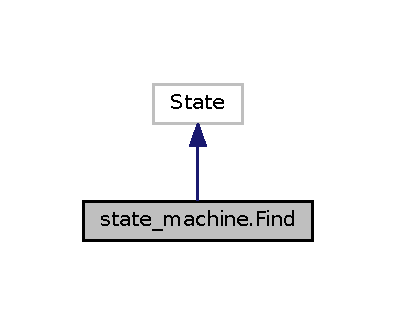
\includegraphics[width=190pt]{classstate__machine_1_1Find__inherit__graph}
\end{center}
\end{figure}


Collaboration diagram for state\+\_\+machine.\+Find\+:
\nopagebreak
\begin{figure}[H]
\begin{center}
\leavevmode
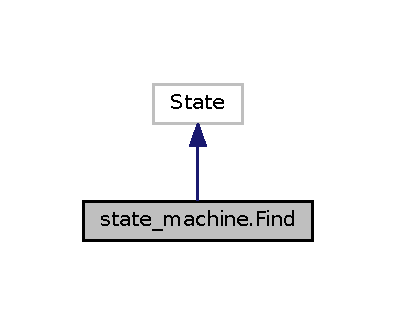
\includegraphics[width=190pt]{classstate__machine_1_1Find__coll__graph}
\end{center}
\end{figure}
\subsection*{Public Member Functions}
\begin{DoxyCompactItemize}
\item 
def \hyperlink{classstate__machine_1_1Find_aa7bd4d07590561e39233a3759ee25f49}{\+\_\+\+\_\+init\+\_\+\+\_\+} (self)
\begin{DoxyCompactList}\small\item\em method init \end{DoxyCompactList}\item 
def \hyperlink{classstate__machine_1_1Find_aa79a6408d288a202d766d86a34d26c22}{execute} (self, userdata)
\item 
def \hyperlink{classstate__machine_1_1Find_a41dd475617a4acb8b239b404257eacb1}{callback} (self, ros\+\_\+data)
\begin{DoxyCompactList}\small\item\em method callback \end{DoxyCompactList}\item 
def \hyperlink{classstate__machine_1_1Find_a1734b9a46e8cfcd5e5e34f992fcdd06e}{countour\+\_\+opencv} (self, lower, upper, hsv, image\+\_\+np)
\begin{DoxyCompactList}\small\item\em method countour\+\_\+opencv \end{DoxyCompactList}\item 
def \hyperlink{classstate__machine_1_1Find_ae571e4ebd97af2bfcabfc7b674cf53d8}{sub\+\_\+track} (self, cnts, image\+\_\+np, \hyperlink{classstate__machine_1_1Find_abf765d9904bb38e118449b2ebacd140a}{ball\+\_\+visible})
\begin{DoxyCompactList}\small\item\em method sub\+\_\+track \end{DoxyCompactList}\item 
def \hyperlink{classstate__machine_1_1Find_a8a35ffb44cefa8b89c7609d10040de76}{save\+\_\+param} (self, \hyperlink{classstate__machine_1_1Find_abf765d9904bb38e118449b2ebacd140a}{ball\+\_\+visible})
\begin{DoxyCompactList}\small\item\em method save\+\_\+param \end{DoxyCompactList}\end{DoxyCompactItemize}
\subsection*{Public Attributes}
\begin{DoxyCompactItemize}
\item 
\hyperlink{classstate__machine_1_1Find_abf765d9904bb38e118449b2ebacd140a}{ball\+\_\+visible}
\end{DoxyCompactItemize}
\subsection*{Static Public Attributes}
\begin{DoxyCompactItemize}
\item 
\hyperlink{classstate__machine_1_1Find_a03b9653ba644781fbeae01fea8227931}{counter}
\item 
\hyperlink{classstate__machine_1_1Find_a147a928dffe82913a947d06b1da343e4}{param}
\item 
\hyperlink{classstate__machine_1_1Find_a56c334f3d8214ea21e7caf8849e9bb63}{stop\+Flag}
\item 
\hyperlink{classstate__machine_1_1Find_a4c1e9b99c291eea6d2d77e0220cc695c}{play\+\_\+state}
\item 
\hyperlink{classstate__machine_1_1Find_a996c2a2fe2c3ff25e2aad4b87073e7c9}{child}
\item 
\hyperlink{classstate__machine_1_1Find_a39a3aa87baef536803bd7812e37ce24f}{pub\+Vel}
\item 
\hyperlink{classstate__machine_1_1Find_ad0300ceff8872223de0bc6ebf8484070}{Twist}
\item 
\hyperlink{classstate__machine_1_1Find_a264fa9455d4286aa26b670ac87d712ab}{queue\+\_\+size}
\item 
\hyperlink{classstate__machine_1_1Find_ab9bfce719b158c4f931736443eac806d}{subscriber}
\item 
\hyperlink{classstate__machine_1_1Find_ac31d8f1d8f7bee55c09c21d42ca37562}{requested\+\_\+room}
\item 
\hyperlink{classstate__machine_1_1Find_ad284228602a30b744143e35e03e938ce}{t\+\_\+final}
\end{DoxyCompactItemize}


\subsection{Detailed Description}
class Find\+\_\+behavior 

when entering \hyperlink{classstate__machine_1_1Find}{Find} behaviour, the robot moves randomly within the environment once it detect a coloured ball, it enters the substate \hyperlink{classstate__machine_1_1Find}{Find} Track 

\subsection{Constructor \& Destructor Documentation}
\index{state\+\_\+machine\+::\+Find@{state\+\_\+machine\+::\+Find}!\+\_\+\+\_\+init\+\_\+\+\_\+@{\+\_\+\+\_\+init\+\_\+\+\_\+}}
\index{\+\_\+\+\_\+init\+\_\+\+\_\+@{\+\_\+\+\_\+init\+\_\+\+\_\+}!state\+\_\+machine\+::\+Find@{state\+\_\+machine\+::\+Find}}
\subsubsection[{\texorpdfstring{\+\_\+\+\_\+init\+\_\+\+\_\+(self)}{__init__(self)}}]{\setlength{\rightskip}{0pt plus 5cm}def state\+\_\+machine.\+Find.\+\_\+\+\_\+init\+\_\+\+\_\+ (
\begin{DoxyParamCaption}
\item[{}]{self}
\end{DoxyParamCaption}
)}\hypertarget{classstate__machine_1_1Find_aa7bd4d07590561e39233a3759ee25f49}{}\label{classstate__machine_1_1Find_aa7bd4d07590561e39233a3759ee25f49}


method init 

initialization 

\subsection{Member Function Documentation}
\index{state\+\_\+machine\+::\+Find@{state\+\_\+machine\+::\+Find}!callback@{callback}}
\index{callback@{callback}!state\+\_\+machine\+::\+Find@{state\+\_\+machine\+::\+Find}}
\subsubsection[{\texorpdfstring{callback(self, ros\+\_\+data)}{callback(self, ros_data)}}]{\setlength{\rightskip}{0pt plus 5cm}def state\+\_\+machine.\+Find.\+callback (
\begin{DoxyParamCaption}
\item[{}]{self, }
\item[{}]{ros\+\_\+data}
\end{DoxyParamCaption}
)}\hypertarget{classstate__machine_1_1Find_a41dd475617a4acb8b239b404257eacb1}{}\label{classstate__machine_1_1Find_a41dd475617a4acb8b239b404257eacb1}


method callback 

Execute callback everytime e new image is available from the camera. it make uses of open\+CV libraries to track the ball within rooms and save the room position \index{state\+\_\+machine\+::\+Find@{state\+\_\+machine\+::\+Find}!countour\+\_\+opencv@{countour\+\_\+opencv}}
\index{countour\+\_\+opencv@{countour\+\_\+opencv}!state\+\_\+machine\+::\+Find@{state\+\_\+machine\+::\+Find}}
\subsubsection[{\texorpdfstring{countour\+\_\+opencv(self, lower, upper, hsv, image\+\_\+np)}{countour_opencv(self, lower, upper, hsv, image_np)}}]{\setlength{\rightskip}{0pt plus 5cm}def state\+\_\+machine.\+Find.\+countour\+\_\+opencv (
\begin{DoxyParamCaption}
\item[{}]{self, }
\item[{}]{lower, }
\item[{}]{upper, }
\item[{}]{hsv, }
\item[{}]{image\+\_\+np}
\end{DoxyParamCaption}
)}\hypertarget{classstate__machine_1_1Find_a1734b9a46e8cfcd5e5e34f992fcdd06e}{}\label{classstate__machine_1_1Find_a1734b9a46e8cfcd5e5e34f992fcdd06e}


method countour\+\_\+opencv 

used to create masks for colours, and their countours \index{state\+\_\+machine\+::\+Find@{state\+\_\+machine\+::\+Find}!execute@{execute}}
\index{execute@{execute}!state\+\_\+machine\+::\+Find@{state\+\_\+machine\+::\+Find}}
\subsubsection[{\texorpdfstring{execute(self, userdata)}{execute(self, userdata)}}]{\setlength{\rightskip}{0pt plus 5cm}def state\+\_\+machine.\+Find.\+execute (
\begin{DoxyParamCaption}
\item[{}]{self, }
\item[{}]{userdata}
\end{DoxyParamCaption}
)}\hypertarget{classstate__machine_1_1Find_aa79a6408d288a202d766d86a34d26c22}{}\label{classstate__machine_1_1Find_aa79a6408d288a202d766d86a34d26c22}
\index{state\+\_\+machine\+::\+Find@{state\+\_\+machine\+::\+Find}!save\+\_\+param@{save\+\_\+param}}
\index{save\+\_\+param@{save\+\_\+param}!state\+\_\+machine\+::\+Find@{state\+\_\+machine\+::\+Find}}
\subsubsection[{\texorpdfstring{save\+\_\+param(self, ball\+\_\+visible)}{save_param(self, ball_visible)}}]{\setlength{\rightskip}{0pt plus 5cm}def state\+\_\+machine.\+Find.\+save\+\_\+param (
\begin{DoxyParamCaption}
\item[{}]{self, }
\item[{}]{ball\+\_\+visible}
\end{DoxyParamCaption}
)}\hypertarget{classstate__machine_1_1Find_a8a35ffb44cefa8b89c7609d10040de76}{}\label{classstate__machine_1_1Find_a8a35ffb44cefa8b89c7609d10040de76}


method save\+\_\+param 

function to store position of the room \index{state\+\_\+machine\+::\+Find@{state\+\_\+machine\+::\+Find}!sub\+\_\+track@{sub\+\_\+track}}
\index{sub\+\_\+track@{sub\+\_\+track}!state\+\_\+machine\+::\+Find@{state\+\_\+machine\+::\+Find}}
\subsubsection[{\texorpdfstring{sub\+\_\+track(self, cnts, image\+\_\+np, ball\+\_\+visible)}{sub_track(self, cnts, image_np, ball_visible)}}]{\setlength{\rightskip}{0pt plus 5cm}def state\+\_\+machine.\+Find.\+sub\+\_\+track (
\begin{DoxyParamCaption}
\item[{}]{self, }
\item[{}]{cnts, }
\item[{}]{image\+\_\+np, }
\item[{}]{ball\+\_\+visible}
\end{DoxyParamCaption}
)}\hypertarget{classstate__machine_1_1Find_ae571e4ebd97af2bfcabfc7b674cf53d8}{}\label{classstate__machine_1_1Find_ae571e4ebd97af2bfcabfc7b674cf53d8}


method sub\+\_\+track 

This function is executed everytime the robot detects a color object which was not previously detected. The robot moves closer to the detected object. Once done, the reference position of the room is marked as reached and stored as \char`\"{}visited\char`\"{} in the parameter server. 

\subsection{Member Data Documentation}
\index{state\+\_\+machine\+::\+Find@{state\+\_\+machine\+::\+Find}!ball\+\_\+visible@{ball\+\_\+visible}}
\index{ball\+\_\+visible@{ball\+\_\+visible}!state\+\_\+machine\+::\+Find@{state\+\_\+machine\+::\+Find}}
\subsubsection[{\texorpdfstring{ball\+\_\+visible}{ball_visible}}]{\setlength{\rightskip}{0pt plus 5cm}state\+\_\+machine.\+Find.\+ball\+\_\+visible}\hypertarget{classstate__machine_1_1Find_abf765d9904bb38e118449b2ebacd140a}{}\label{classstate__machine_1_1Find_abf765d9904bb38e118449b2ebacd140a}
\index{state\+\_\+machine\+::\+Find@{state\+\_\+machine\+::\+Find}!child@{child}}
\index{child@{child}!state\+\_\+machine\+::\+Find@{state\+\_\+machine\+::\+Find}}
\subsubsection[{\texorpdfstring{child}{child}}]{\setlength{\rightskip}{0pt plus 5cm}state\+\_\+machine.\+Find.\+child\hspace{0.3cm}{\ttfamily [static]}}\hypertarget{classstate__machine_1_1Find_a996c2a2fe2c3ff25e2aad4b87073e7c9}{}\label{classstate__machine_1_1Find_a996c2a2fe2c3ff25e2aad4b87073e7c9}
\index{state\+\_\+machine\+::\+Find@{state\+\_\+machine\+::\+Find}!counter@{counter}}
\index{counter@{counter}!state\+\_\+machine\+::\+Find@{state\+\_\+machine\+::\+Find}}
\subsubsection[{\texorpdfstring{counter}{counter}}]{\setlength{\rightskip}{0pt plus 5cm}state\+\_\+machine.\+Find.\+counter\hspace{0.3cm}{\ttfamily [static]}}\hypertarget{classstate__machine_1_1Find_a03b9653ba644781fbeae01fea8227931}{}\label{classstate__machine_1_1Find_a03b9653ba644781fbeae01fea8227931}
\index{state\+\_\+machine\+::\+Find@{state\+\_\+machine\+::\+Find}!param@{param}}
\index{param@{param}!state\+\_\+machine\+::\+Find@{state\+\_\+machine\+::\+Find}}
\subsubsection[{\texorpdfstring{param}{param}}]{\setlength{\rightskip}{0pt plus 5cm}state\+\_\+machine.\+Find.\+param\hspace{0.3cm}{\ttfamily [static]}}\hypertarget{classstate__machine_1_1Find_a147a928dffe82913a947d06b1da343e4}{}\label{classstate__machine_1_1Find_a147a928dffe82913a947d06b1da343e4}
\index{state\+\_\+machine\+::\+Find@{state\+\_\+machine\+::\+Find}!play\+\_\+state@{play\+\_\+state}}
\index{play\+\_\+state@{play\+\_\+state}!state\+\_\+machine\+::\+Find@{state\+\_\+machine\+::\+Find}}
\subsubsection[{\texorpdfstring{play\+\_\+state}{play_state}}]{\setlength{\rightskip}{0pt plus 5cm}state\+\_\+machine.\+Find.\+play\+\_\+state\hspace{0.3cm}{\ttfamily [static]}}\hypertarget{classstate__machine_1_1Find_a4c1e9b99c291eea6d2d77e0220cc695c}{}\label{classstate__machine_1_1Find_a4c1e9b99c291eea6d2d77e0220cc695c}
\index{state\+\_\+machine\+::\+Find@{state\+\_\+machine\+::\+Find}!pub\+Vel@{pub\+Vel}}
\index{pub\+Vel@{pub\+Vel}!state\+\_\+machine\+::\+Find@{state\+\_\+machine\+::\+Find}}
\subsubsection[{\texorpdfstring{pub\+Vel}{pubVel}}]{\setlength{\rightskip}{0pt plus 5cm}state\+\_\+machine.\+Find.\+pub\+Vel\hspace{0.3cm}{\ttfamily [static]}}\hypertarget{classstate__machine_1_1Find_a39a3aa87baef536803bd7812e37ce24f}{}\label{classstate__machine_1_1Find_a39a3aa87baef536803bd7812e37ce24f}
\index{state\+\_\+machine\+::\+Find@{state\+\_\+machine\+::\+Find}!queue\+\_\+size@{queue\+\_\+size}}
\index{queue\+\_\+size@{queue\+\_\+size}!state\+\_\+machine\+::\+Find@{state\+\_\+machine\+::\+Find}}
\subsubsection[{\texorpdfstring{queue\+\_\+size}{queue_size}}]{\setlength{\rightskip}{0pt plus 5cm}state\+\_\+machine.\+Find.\+queue\+\_\+size\hspace{0.3cm}{\ttfamily [static]}}\hypertarget{classstate__machine_1_1Find_a264fa9455d4286aa26b670ac87d712ab}{}\label{classstate__machine_1_1Find_a264fa9455d4286aa26b670ac87d712ab}
\index{state\+\_\+machine\+::\+Find@{state\+\_\+machine\+::\+Find}!requested\+\_\+room@{requested\+\_\+room}}
\index{requested\+\_\+room@{requested\+\_\+room}!state\+\_\+machine\+::\+Find@{state\+\_\+machine\+::\+Find}}
\subsubsection[{\texorpdfstring{requested\+\_\+room}{requested_room}}]{\setlength{\rightskip}{0pt plus 5cm}state\+\_\+machine.\+Find.\+requested\+\_\+room\hspace{0.3cm}{\ttfamily [static]}}\hypertarget{classstate__machine_1_1Find_ac31d8f1d8f7bee55c09c21d42ca37562}{}\label{classstate__machine_1_1Find_ac31d8f1d8f7bee55c09c21d42ca37562}
\index{state\+\_\+machine\+::\+Find@{state\+\_\+machine\+::\+Find}!stop\+Flag@{stop\+Flag}}
\index{stop\+Flag@{stop\+Flag}!state\+\_\+machine\+::\+Find@{state\+\_\+machine\+::\+Find}}
\subsubsection[{\texorpdfstring{stop\+Flag}{stopFlag}}]{\setlength{\rightskip}{0pt plus 5cm}state\+\_\+machine.\+Find.\+stop\+Flag\hspace{0.3cm}{\ttfamily [static]}}\hypertarget{classstate__machine_1_1Find_a56c334f3d8214ea21e7caf8849e9bb63}{}\label{classstate__machine_1_1Find_a56c334f3d8214ea21e7caf8849e9bb63}
\index{state\+\_\+machine\+::\+Find@{state\+\_\+machine\+::\+Find}!subscriber@{subscriber}}
\index{subscriber@{subscriber}!state\+\_\+machine\+::\+Find@{state\+\_\+machine\+::\+Find}}
\subsubsection[{\texorpdfstring{subscriber}{subscriber}}]{\setlength{\rightskip}{0pt plus 5cm}state\+\_\+machine.\+Find.\+subscriber\hspace{0.3cm}{\ttfamily [static]}}\hypertarget{classstate__machine_1_1Find_ab9bfce719b158c4f931736443eac806d}{}\label{classstate__machine_1_1Find_ab9bfce719b158c4f931736443eac806d}
{\bfseries Initial value\+:}
\begin{DoxyCode}
1 = rospy.Subscriber(\textcolor{stringliteral}{"camera1/image\_raw/compressed"},
2                                               CompressedImage, self.callback,  queue\_size=1)
\end{DoxyCode}
\index{state\+\_\+machine\+::\+Find@{state\+\_\+machine\+::\+Find}!t\+\_\+final@{t\+\_\+final}}
\index{t\+\_\+final@{t\+\_\+final}!state\+\_\+machine\+::\+Find@{state\+\_\+machine\+::\+Find}}
\subsubsection[{\texorpdfstring{t\+\_\+final}{t_final}}]{\setlength{\rightskip}{0pt plus 5cm}state\+\_\+machine.\+Find.\+t\+\_\+final\hspace{0.3cm}{\ttfamily [static]}}\hypertarget{classstate__machine_1_1Find_ad284228602a30b744143e35e03e938ce}{}\label{classstate__machine_1_1Find_ad284228602a30b744143e35e03e938ce}
\index{state\+\_\+machine\+::\+Find@{state\+\_\+machine\+::\+Find}!Twist@{Twist}}
\index{Twist@{Twist}!state\+\_\+machine\+::\+Find@{state\+\_\+machine\+::\+Find}}
\subsubsection[{\texorpdfstring{Twist}{Twist}}]{\setlength{\rightskip}{0pt plus 5cm}state\+\_\+machine.\+Find.\+Twist\hspace{0.3cm}{\ttfamily [static]}}\hypertarget{classstate__machine_1_1Find_ad0300ceff8872223de0bc6ebf8484070}{}\label{classstate__machine_1_1Find_ad0300ceff8872223de0bc6ebf8484070}


The documentation for this class was generated from the following file\+:\begin{DoxyCompactItemize}
\item 
/home/\+Experimental\+Robotics\+Lab\+Serena/src/final\+\_\+assignment/scripts/\hyperlink{state__machine_8py}{state\+\_\+machine.\+py}\end{DoxyCompactItemize}

\hypertarget{classstate__machine_1_1Normal}{}\section{state\+\_\+machine.\+Normal Class Reference}
\label{classstate__machine_1_1Normal}\index{state\+\_\+machine.\+Normal@{state\+\_\+machine.\+Normal}}


class Normal\+\_\+behavior  




Inheritance diagram for state\+\_\+machine.\+Normal\+:
\nopagebreak
\begin{figure}[H]
\begin{center}
\leavevmode
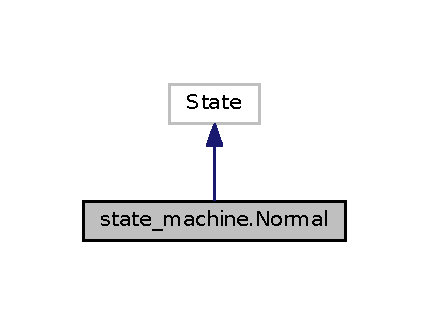
\includegraphics[width=206pt]{classstate__machine_1_1Normal__inherit__graph}
\end{center}
\end{figure}


Collaboration diagram for state\+\_\+machine.\+Normal\+:
\nopagebreak
\begin{figure}[H]
\begin{center}
\leavevmode
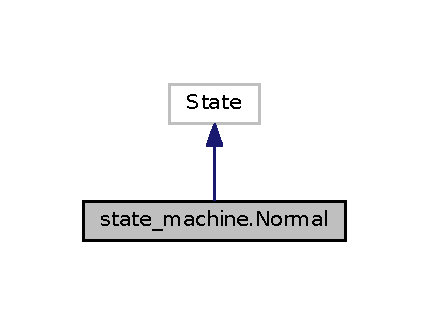
\includegraphics[width=206pt]{classstate__machine_1_1Normal__coll__graph}
\end{center}
\end{figure}
\subsection*{Public Member Functions}
\begin{DoxyCompactItemize}
\item 
def \hyperlink{classstate__machine_1_1Normal_acdbc35a37d0350d7805a628048bc3bed}{\+\_\+\+\_\+init\+\_\+\+\_\+} (self)
\begin{DoxyCompactList}\small\item\em method init \end{DoxyCompactList}\item 
def \hyperlink{classstate__machine_1_1Normal_a2930df5f4890ec4b47b2a8e18f9bff08}{execute} (self, userdata)
\begin{DoxyCompactList}\small\item\em method execute \end{DoxyCompactList}\item 
def \hyperlink{classstate__machine_1_1Normal_a9e1b8d69a0e55eff3518dae91a81626a}{robot\+\_\+vel} (self, msg)
\begin{DoxyCompactList}\small\item\em function robot\+\_\+vel \end{DoxyCompactList}\item 
def \hyperlink{classstate__machine_1_1Normal_ab8bc608e9dab104a02f5ef47b4420aa3}{callback} (self, ros\+\_\+data)
\begin{DoxyCompactList}\small\item\em method callback \end{DoxyCompactList}\item 
def \hyperlink{classstate__machine_1_1Normal_ae850fe2a131b73c9b558780700411e98}{countour\+\_\+opencv} (self, lower, upper, hsv, image\+\_\+np)
\begin{DoxyCompactList}\small\item\em method countour\+\_\+opencv \end{DoxyCompactList}\item 
def \hyperlink{classstate__machine_1_1Normal_a2bcff58a537d46bdb548c4fa3eb1f2c8}{sub\+\_\+track} (self, cnts, image\+\_\+np, \hyperlink{classstate__machine_1_1Normal_aa7f6732a154ed8e53353598c2278cd49}{ball\+\_\+visible})
\begin{DoxyCompactList}\small\item\em method sub\+\_\+track \end{DoxyCompactList}\item 
def \hyperlink{classstate__machine_1_1Normal_a00b62ef4a75771f3a13cbc8c0a3e0387}{save\+\_\+param} (self, \hyperlink{classstate__machine_1_1Normal_aa7f6732a154ed8e53353598c2278cd49}{ball\+\_\+visible})
\begin{DoxyCompactList}\small\item\em method save\+\_\+param \end{DoxyCompactList}\end{DoxyCompactItemize}
\subsection*{Static Public Attributes}
\begin{DoxyCompactItemize}
\item 
\hyperlink{classstate__machine_1_1Normal_a4b32c1a56ad043f9913b9b3068aafaa1}{counter\+Sleep}
\item 
\hyperlink{classstate__machine_1_1Normal_ad9306b3db821d9634339a20308e48a25}{counter\+Play}
\begin{DoxyCompactList}\small\item\em counters to switch behavior \end{DoxyCompactList}\item 
\hyperlink{classstate__machine_1_1Normal_ad631fe332b431c0001682701dde8dbed}{counter}
\item 
\hyperlink{classstate__machine_1_1Normal_a27eca8cdd2bee790ad3eecd42c23e3b5}{stop\+Flag}
\item 
\hyperlink{classstate__machine_1_1Normal_ad676a7bddfcb08e695d05338b57989f9}{param}
\item 
\hyperlink{classstate__machine_1_1Normal_aa7f6732a154ed8e53353598c2278cd49}{ball\+\_\+visible}
\item 
\hyperlink{classstate__machine_1_1Normal_ab6d144a3dda6248e1d2f30f9abe9d609}{outcomes}
\item 
\hyperlink{classstate__machine_1_1Normal_abf3086095a488112b289e23941a57809}{pub\+Goal} = rospy.\+Publisher(\textquotesingle{}goal\+Pos\textquotesingle{}, Num, \hyperlink{classstate__machine_1_1Normal_ae4b7ade70a0e23f0dd8738aaca0b4e4d}{queue\+\_\+size} = 10)
\begin{DoxyCompactList}\small\item\em publishers / subscribers publisher to topic /goal\+Pos \end{DoxyCompactList}\item 
\hyperlink{classstate__machine_1_1Normal_a12658175f11bf60d621652d845da5d31}{sub\+Vel} = rospy.\+Subscriber(\char`\"{}cmd\+\_\+vel\char`\"{}, Twist, self.\+robot\+\_\+vel)
\item 
\hyperlink{classstate__machine_1_1Normal_a8f98c449693c58319157bc51e2621157}{pub\+Vel}
\item 
\hyperlink{classstate__machine_1_1Normal_a6f6f347ff2c917d80cdb28f42e7cfd47}{Twist}
\item 
\hyperlink{classstate__machine_1_1Normal_ae4b7ade70a0e23f0dd8738aaca0b4e4d}{queue\+\_\+size}
\item 
\hyperlink{classstate__machine_1_1Normal_a813c3112edc54d4146e8c07ef6f7e040}{sub\+Cam}
\item 
\hyperlink{classstate__machine_1_1Normal_a9696c713d102313a01209dce8e05aea3}{var}
\item 
\hyperlink{classstate__machine_1_1Normal_ac4a9f6b5f01a6edbde7d181dea3bd92a}{randomlist} = \hyperlink{namespacestate__machine_ad624b5f98b8358f20b7cecc4b88c9f52}{random\+\_\+position}()
\begin{DoxyCompactList}\small\item\em send the robot to a random goal positions compute random position with function \hyperlink{namespacestate__machine_ad624b5f98b8358f20b7cecc4b88c9f52}{random\+\_\+position()} \end{DoxyCompactList}\item 
\hyperlink{classstate__machine_1_1Normal_a9e0c7641755e2614e74b3228fbef0a82}{c} = max(cnts, key = cv2.\+contour\+Area)
\item 
\hyperlink{classstate__machine_1_1Normal_afa87ced0c5fa2d65c957a16bd517fc39}{radius}
\item 
\hyperlink{classstate__machine_1_1Normal_a8b720e4cdaf1aff877cc16eb72887ca4}{M} = cv2.\+moments(\hyperlink{classstate__machine_1_1Normal_a9e0c7641755e2614e74b3228fbef0a82}{c})
\item 
tuple \hyperlink{classstate__machine_1_1Normal_a91a5741f842196647b0f7267ce568aeb}{center} = (int(\hyperlink{classstate__machine_1_1Normal_a8b720e4cdaf1aff877cc16eb72887ca4}{M}\mbox{[}\char`\"{}m10\char`\"{}\mbox{]} / M\mbox{[}\char`\"{}m00\char`\"{}\mbox{]}), int(\hyperlink{classstate__machine_1_1Normal_a8b720e4cdaf1aff877cc16eb72887ca4}{M}\mbox{[}\char`\"{}m01\char`\"{}\mbox{]} / M\mbox{[}\char`\"{}m00\char`\"{}\mbox{]}))
\item 
\hyperlink{classstate__machine_1_1Normal_aa1d4a50c677406423e29048758a79596}{vel} = \hyperlink{classstate__machine_1_1Normal_a6f6f347ff2c917d80cdb28f42e7cfd47}{Twist}()
\item 
\hyperlink{classstate__machine_1_1Normal_a6261e388441dd73175646b4eb06453f7}{z}
\item 
\hyperlink{classstate__machine_1_1Normal_a474c7681d4377c15bf89a5062887bd49}{x}
\end{DoxyCompactItemize}


\subsection{Detailed Description}
class Normal\+\_\+behavior 

This class implement the N\+O\+R\+M\+AL behaviour of the robot pet The robot moves randomly within the Gazebo arena
\begin{DoxyItemize}
\item If it receives a \char`\"{}play\char`\"{} command the F\+SM should go into P\+L\+AY state (start\+\_\+play)
\item If the sleep timer is triggered the F\+SM should go into S\+L\+E\+EP state (start\+\_\+sleep) 
\end{DoxyItemize}

\subsection{Constructor \& Destructor Documentation}
\index{state\+\_\+machine\+::\+Normal@{state\+\_\+machine\+::\+Normal}!\+\_\+\+\_\+init\+\_\+\+\_\+@{\+\_\+\+\_\+init\+\_\+\+\_\+}}
\index{\+\_\+\+\_\+init\+\_\+\+\_\+@{\+\_\+\+\_\+init\+\_\+\+\_\+}!state\+\_\+machine\+::\+Normal@{state\+\_\+machine\+::\+Normal}}
\subsubsection[{\texorpdfstring{\+\_\+\+\_\+init\+\_\+\+\_\+(self)}{__init__(self)}}]{\setlength{\rightskip}{0pt plus 5cm}def state\+\_\+machine.\+Normal.\+\_\+\+\_\+init\+\_\+\+\_\+ (
\begin{DoxyParamCaption}
\item[{}]{self}
\end{DoxyParamCaption}
)}\hypertarget{classstate__machine_1_1Normal_acdbc35a37d0350d7805a628048bc3bed}{}\label{classstate__machine_1_1Normal_acdbc35a37d0350d7805a628048bc3bed}


method init 

This method should\+:
\begin{DoxyItemize}
\item initializes the state class 
\end{DoxyItemize}

\subsection{Member Function Documentation}
\index{state\+\_\+machine\+::\+Normal@{state\+\_\+machine\+::\+Normal}!callback@{callback}}
\index{callback@{callback}!state\+\_\+machine\+::\+Normal@{state\+\_\+machine\+::\+Normal}}
\subsubsection[{\texorpdfstring{callback(self, ros\+\_\+data)}{callback(self, ros_data)}}]{\setlength{\rightskip}{0pt plus 5cm}def state\+\_\+machine.\+Normal.\+callback (
\begin{DoxyParamCaption}
\item[{}]{self, }
\item[{}]{ros\+\_\+data}
\end{DoxyParamCaption}
)}\hypertarget{classstate__machine_1_1Normal_ab8bc608e9dab104a02f5ef47b4420aa3}{}\label{classstate__machine_1_1Normal_ab8bc608e9dab104a02f5ef47b4420aa3}


method callback 

Execute callback everytime e new image is available from the camera. it make uses of open\+CV libraries to track the ball within rooms and save the room position it calls methods\+:
\begin{DoxyItemize}
\item countour\+\_\+opencv
\item sub\+\_\+track 
\end{DoxyItemize}\index{state\+\_\+machine\+::\+Normal@{state\+\_\+machine\+::\+Normal}!countour\+\_\+opencv@{countour\+\_\+opencv}}
\index{countour\+\_\+opencv@{countour\+\_\+opencv}!state\+\_\+machine\+::\+Normal@{state\+\_\+machine\+::\+Normal}}
\subsubsection[{\texorpdfstring{countour\+\_\+opencv(self, lower, upper, hsv, image\+\_\+np)}{countour_opencv(self, lower, upper, hsv, image_np)}}]{\setlength{\rightskip}{0pt plus 5cm}def state\+\_\+machine.\+Normal.\+countour\+\_\+opencv (
\begin{DoxyParamCaption}
\item[{}]{self, }
\item[{}]{lower, }
\item[{}]{upper, }
\item[{}]{hsv, }
\item[{}]{image\+\_\+np}
\end{DoxyParamCaption}
)}\hypertarget{classstate__machine_1_1Normal_ae850fe2a131b73c9b558780700411e98}{}\label{classstate__machine_1_1Normal_ae850fe2a131b73c9b558780700411e98}


method countour\+\_\+opencv 

used to create masks for colours, and their countours \index{state\+\_\+machine\+::\+Normal@{state\+\_\+machine\+::\+Normal}!execute@{execute}}
\index{execute@{execute}!state\+\_\+machine\+::\+Normal@{state\+\_\+machine\+::\+Normal}}
\subsubsection[{\texorpdfstring{execute(self, userdata)}{execute(self, userdata)}}]{\setlength{\rightskip}{0pt plus 5cm}def state\+\_\+machine.\+Normal.\+execute (
\begin{DoxyParamCaption}
\item[{}]{self, }
\item[{}]{userdata}
\end{DoxyParamCaption}
)}\hypertarget{classstate__machine_1_1Normal_a2930df5f4890ec4b47b2a8e18f9bff08}{}\label{classstate__machine_1_1Normal_a2930df5f4890ec4b47b2a8e18f9bff08}


method execute 

This method\+:
\begin{DoxyItemize}
\item robot moves randomly within the map
\item to do so, we sent random goal positions he has to reach
\item when it detects a coloured object within the camera range it runs the callback method
\item this callback implements a opencv algorithm to detect objects
\item once detected it enters T\+R\+A\+CK substate to get closer to the ball and save the room position 
\end{DoxyItemize}\index{state\+\_\+machine\+::\+Normal@{state\+\_\+machine\+::\+Normal}!robot\+\_\+vel@{robot\+\_\+vel}}
\index{robot\+\_\+vel@{robot\+\_\+vel}!state\+\_\+machine\+::\+Normal@{state\+\_\+machine\+::\+Normal}}
\subsubsection[{\texorpdfstring{robot\+\_\+vel(self, msg)}{robot_vel(self, msg)}}]{\setlength{\rightskip}{0pt plus 5cm}def state\+\_\+machine.\+Normal.\+robot\+\_\+vel (
\begin{DoxyParamCaption}
\item[{}]{self, }
\item[{}]{msg}
\end{DoxyParamCaption}
)}\hypertarget{classstate__machine_1_1Normal_a9e1b8d69a0e55eff3518dae91a81626a}{}\label{classstate__machine_1_1Normal_a9e1b8d69a0e55eff3518dae91a81626a}


function robot\+\_\+vel 

callback to check if the robot is moving or not A flag is set to 1 if the robot is not moving, to 0 otherwise \index{state\+\_\+machine\+::\+Normal@{state\+\_\+machine\+::\+Normal}!save\+\_\+param@{save\+\_\+param}}
\index{save\+\_\+param@{save\+\_\+param}!state\+\_\+machine\+::\+Normal@{state\+\_\+machine\+::\+Normal}}
\subsubsection[{\texorpdfstring{save\+\_\+param(self, ball\+\_\+visible)}{save_param(self, ball_visible)}}]{\setlength{\rightskip}{0pt plus 5cm}def state\+\_\+machine.\+Normal.\+save\+\_\+param (
\begin{DoxyParamCaption}
\item[{}]{self, }
\item[{}]{ball\+\_\+visible}
\end{DoxyParamCaption}
)}\hypertarget{classstate__machine_1_1Normal_a00b62ef4a75771f3a13cbc8c0a3e0387}{}\label{classstate__machine_1_1Normal_a00b62ef4a75771f3a13cbc8c0a3e0387}


method save\+\_\+param 

function to store position of the room \index{state\+\_\+machine\+::\+Normal@{state\+\_\+machine\+::\+Normal}!sub\+\_\+track@{sub\+\_\+track}}
\index{sub\+\_\+track@{sub\+\_\+track}!state\+\_\+machine\+::\+Normal@{state\+\_\+machine\+::\+Normal}}
\subsubsection[{\texorpdfstring{sub\+\_\+track(self, cnts, image\+\_\+np, ball\+\_\+visible)}{sub_track(self, cnts, image_np, ball_visible)}}]{\setlength{\rightskip}{0pt plus 5cm}def state\+\_\+machine.\+Normal.\+sub\+\_\+track (
\begin{DoxyParamCaption}
\item[{}]{self, }
\item[{}]{cnts, }
\item[{}]{image\+\_\+np, }
\item[{}]{ball\+\_\+visible}
\end{DoxyParamCaption}
)}\hypertarget{classstate__machine_1_1Normal_a2bcff58a537d46bdb548c4fa3eb1f2c8}{}\label{classstate__machine_1_1Normal_a2bcff58a537d46bdb548c4fa3eb1f2c8}


method sub\+\_\+track 

This function is executed everytime the robot detects a color object which was not previously detected. The robot moves closer to the detected object. Once done, the reference position of the room is marked as reached and stored as \char`\"{}visited\char`\"{} in the parameter server. 

\subsection{Member Data Documentation}
\index{state\+\_\+machine\+::\+Normal@{state\+\_\+machine\+::\+Normal}!ball\+\_\+visible@{ball\+\_\+visible}}
\index{ball\+\_\+visible@{ball\+\_\+visible}!state\+\_\+machine\+::\+Normal@{state\+\_\+machine\+::\+Normal}}
\subsubsection[{\texorpdfstring{ball\+\_\+visible}{ball_visible}}]{\setlength{\rightskip}{0pt plus 5cm}state\+\_\+machine.\+Normal.\+ball\+\_\+visible\hspace{0.3cm}{\ttfamily [static]}}\hypertarget{classstate__machine_1_1Normal_aa7f6732a154ed8e53353598c2278cd49}{}\label{classstate__machine_1_1Normal_aa7f6732a154ed8e53353598c2278cd49}
\index{state\+\_\+machine\+::\+Normal@{state\+\_\+machine\+::\+Normal}!c@{c}}
\index{c@{c}!state\+\_\+machine\+::\+Normal@{state\+\_\+machine\+::\+Normal}}
\subsubsection[{\texorpdfstring{c}{c}}]{\setlength{\rightskip}{0pt plus 5cm}state\+\_\+machine.\+Normal.\+c = max(cnts, key = cv2.\+contour\+Area)\hspace{0.3cm}{\ttfamily [static]}}\hypertarget{classstate__machine_1_1Normal_a9e0c7641755e2614e74b3228fbef0a82}{}\label{classstate__machine_1_1Normal_a9e0c7641755e2614e74b3228fbef0a82}
\index{state\+\_\+machine\+::\+Normal@{state\+\_\+machine\+::\+Normal}!center@{center}}
\index{center@{center}!state\+\_\+machine\+::\+Normal@{state\+\_\+machine\+::\+Normal}}
\subsubsection[{\texorpdfstring{center}{center}}]{\setlength{\rightskip}{0pt plus 5cm}tuple state\+\_\+machine.\+Normal.\+center = (int({\bf M}\mbox{[}\char`\"{}m10\char`\"{}\mbox{]} / M\mbox{[}\char`\"{}m00\char`\"{}\mbox{]}), int({\bf M}\mbox{[}\char`\"{}m01\char`\"{}\mbox{]} / M\mbox{[}\char`\"{}m00\char`\"{}\mbox{]}))\hspace{0.3cm}{\ttfamily [static]}}\hypertarget{classstate__machine_1_1Normal_a91a5741f842196647b0f7267ce568aeb}{}\label{classstate__machine_1_1Normal_a91a5741f842196647b0f7267ce568aeb}
\index{state\+\_\+machine\+::\+Normal@{state\+\_\+machine\+::\+Normal}!counter@{counter}}
\index{counter@{counter}!state\+\_\+machine\+::\+Normal@{state\+\_\+machine\+::\+Normal}}
\subsubsection[{\texorpdfstring{counter}{counter}}]{\setlength{\rightskip}{0pt plus 5cm}state\+\_\+machine.\+Normal.\+counter\hspace{0.3cm}{\ttfamily [static]}}\hypertarget{classstate__machine_1_1Normal_ad631fe332b431c0001682701dde8dbed}{}\label{classstate__machine_1_1Normal_ad631fe332b431c0001682701dde8dbed}
\index{state\+\_\+machine\+::\+Normal@{state\+\_\+machine\+::\+Normal}!counter\+Play@{counter\+Play}}
\index{counter\+Play@{counter\+Play}!state\+\_\+machine\+::\+Normal@{state\+\_\+machine\+::\+Normal}}
\subsubsection[{\texorpdfstring{counter\+Play}{counterPlay}}]{\setlength{\rightskip}{0pt plus 5cm}state\+\_\+machine.\+Normal.\+counter\+Play\hspace{0.3cm}{\ttfamily [static]}}\hypertarget{classstate__machine_1_1Normal_ad9306b3db821d9634339a20308e48a25}{}\label{classstate__machine_1_1Normal_ad9306b3db821d9634339a20308e48a25}


counters to switch behavior 

\index{state\+\_\+machine\+::\+Normal@{state\+\_\+machine\+::\+Normal}!counter\+Sleep@{counter\+Sleep}}
\index{counter\+Sleep@{counter\+Sleep}!state\+\_\+machine\+::\+Normal@{state\+\_\+machine\+::\+Normal}}
\subsubsection[{\texorpdfstring{counter\+Sleep}{counterSleep}}]{\setlength{\rightskip}{0pt plus 5cm}state\+\_\+machine.\+Normal.\+counter\+Sleep\hspace{0.3cm}{\ttfamily [static]}}\hypertarget{classstate__machine_1_1Normal_a4b32c1a56ad043f9913b9b3068aafaa1}{}\label{classstate__machine_1_1Normal_a4b32c1a56ad043f9913b9b3068aafaa1}
\index{state\+\_\+machine\+::\+Normal@{state\+\_\+machine\+::\+Normal}!M@{M}}
\index{M@{M}!state\+\_\+machine\+::\+Normal@{state\+\_\+machine\+::\+Normal}}
\subsubsection[{\texorpdfstring{M}{M}}]{\setlength{\rightskip}{0pt plus 5cm}state\+\_\+machine.\+Normal.\+M = cv2.\+moments({\bf c})\hspace{0.3cm}{\ttfamily [static]}}\hypertarget{classstate__machine_1_1Normal_a8b720e4cdaf1aff877cc16eb72887ca4}{}\label{classstate__machine_1_1Normal_a8b720e4cdaf1aff877cc16eb72887ca4}
\index{state\+\_\+machine\+::\+Normal@{state\+\_\+machine\+::\+Normal}!outcomes@{outcomes}}
\index{outcomes@{outcomes}!state\+\_\+machine\+::\+Normal@{state\+\_\+machine\+::\+Normal}}
\subsubsection[{\texorpdfstring{outcomes}{outcomes}}]{\setlength{\rightskip}{0pt plus 5cm}state\+\_\+machine.\+Normal.\+outcomes\hspace{0.3cm}{\ttfamily [static]}}\hypertarget{classstate__machine_1_1Normal_ab6d144a3dda6248e1d2f30f9abe9d609}{}\label{classstate__machine_1_1Normal_ab6d144a3dda6248e1d2f30f9abe9d609}
\index{state\+\_\+machine\+::\+Normal@{state\+\_\+machine\+::\+Normal}!param@{param}}
\index{param@{param}!state\+\_\+machine\+::\+Normal@{state\+\_\+machine\+::\+Normal}}
\subsubsection[{\texorpdfstring{param}{param}}]{\setlength{\rightskip}{0pt plus 5cm}state\+\_\+machine.\+Normal.\+param\hspace{0.3cm}{\ttfamily [static]}}\hypertarget{classstate__machine_1_1Normal_ad676a7bddfcb08e695d05338b57989f9}{}\label{classstate__machine_1_1Normal_ad676a7bddfcb08e695d05338b57989f9}
\index{state\+\_\+machine\+::\+Normal@{state\+\_\+machine\+::\+Normal}!pub\+Goal@{pub\+Goal}}
\index{pub\+Goal@{pub\+Goal}!state\+\_\+machine\+::\+Normal@{state\+\_\+machine\+::\+Normal}}
\subsubsection[{\texorpdfstring{pub\+Goal}{pubGoal}}]{\setlength{\rightskip}{0pt plus 5cm}state\+\_\+machine.\+Normal.\+pub\+Goal = rospy.\+Publisher(\textquotesingle{}goal\+Pos\textquotesingle{}, Num, {\bf queue\+\_\+size} = 10)\hspace{0.3cm}{\ttfamily [static]}}\hypertarget{classstate__machine_1_1Normal_abf3086095a488112b289e23941a57809}{}\label{classstate__machine_1_1Normal_abf3086095a488112b289e23941a57809}


publishers / subscribers publisher to topic /goal\+Pos 

\index{state\+\_\+machine\+::\+Normal@{state\+\_\+machine\+::\+Normal}!pub\+Vel@{pub\+Vel}}
\index{pub\+Vel@{pub\+Vel}!state\+\_\+machine\+::\+Normal@{state\+\_\+machine\+::\+Normal}}
\subsubsection[{\texorpdfstring{pub\+Vel}{pubVel}}]{\setlength{\rightskip}{0pt plus 5cm}state\+\_\+machine.\+Normal.\+pub\+Vel\hspace{0.3cm}{\ttfamily [static]}}\hypertarget{classstate__machine_1_1Normal_a8f98c449693c58319157bc51e2621157}{}\label{classstate__machine_1_1Normal_a8f98c449693c58319157bc51e2621157}
\index{state\+\_\+machine\+::\+Normal@{state\+\_\+machine\+::\+Normal}!queue\+\_\+size@{queue\+\_\+size}}
\index{queue\+\_\+size@{queue\+\_\+size}!state\+\_\+machine\+::\+Normal@{state\+\_\+machine\+::\+Normal}}
\subsubsection[{\texorpdfstring{queue\+\_\+size}{queue_size}}]{\setlength{\rightskip}{0pt plus 5cm}state\+\_\+machine.\+Normal.\+queue\+\_\+size\hspace{0.3cm}{\ttfamily [static]}}\hypertarget{classstate__machine_1_1Normal_ae4b7ade70a0e23f0dd8738aaca0b4e4d}{}\label{classstate__machine_1_1Normal_ae4b7ade70a0e23f0dd8738aaca0b4e4d}
\index{state\+\_\+machine\+::\+Normal@{state\+\_\+machine\+::\+Normal}!radius@{radius}}
\index{radius@{radius}!state\+\_\+machine\+::\+Normal@{state\+\_\+machine\+::\+Normal}}
\subsubsection[{\texorpdfstring{radius}{radius}}]{\setlength{\rightskip}{0pt plus 5cm}state\+\_\+machine.\+Normal.\+radius\hspace{0.3cm}{\ttfamily [static]}}\hypertarget{classstate__machine_1_1Normal_afa87ced0c5fa2d65c957a16bd517fc39}{}\label{classstate__machine_1_1Normal_afa87ced0c5fa2d65c957a16bd517fc39}
\index{state\+\_\+machine\+::\+Normal@{state\+\_\+machine\+::\+Normal}!randomlist@{randomlist}}
\index{randomlist@{randomlist}!state\+\_\+machine\+::\+Normal@{state\+\_\+machine\+::\+Normal}}
\subsubsection[{\texorpdfstring{randomlist}{randomlist}}]{\setlength{\rightskip}{0pt plus 5cm}state\+\_\+machine.\+Normal.\+randomlist = {\bf random\+\_\+position}()\hspace{0.3cm}{\ttfamily [static]}}\hypertarget{classstate__machine_1_1Normal_ac4a9f6b5f01a6edbde7d181dea3bd92a}{}\label{classstate__machine_1_1Normal_ac4a9f6b5f01a6edbde7d181dea3bd92a}


send the robot to a random goal positions compute random position with function \hyperlink{namespacestate__machine_ad624b5f98b8358f20b7cecc4b88c9f52}{random\+\_\+position()} 

\index{state\+\_\+machine\+::\+Normal@{state\+\_\+machine\+::\+Normal}!stop\+Flag@{stop\+Flag}}
\index{stop\+Flag@{stop\+Flag}!state\+\_\+machine\+::\+Normal@{state\+\_\+machine\+::\+Normal}}
\subsubsection[{\texorpdfstring{stop\+Flag}{stopFlag}}]{\setlength{\rightskip}{0pt plus 5cm}state\+\_\+machine.\+Normal.\+stop\+Flag\hspace{0.3cm}{\ttfamily [static]}}\hypertarget{classstate__machine_1_1Normal_a27eca8cdd2bee790ad3eecd42c23e3b5}{}\label{classstate__machine_1_1Normal_a27eca8cdd2bee790ad3eecd42c23e3b5}
\index{state\+\_\+machine\+::\+Normal@{state\+\_\+machine\+::\+Normal}!sub\+Cam@{sub\+Cam}}
\index{sub\+Cam@{sub\+Cam}!state\+\_\+machine\+::\+Normal@{state\+\_\+machine\+::\+Normal}}
\subsubsection[{\texorpdfstring{sub\+Cam}{subCam}}]{\setlength{\rightskip}{0pt plus 5cm}state\+\_\+machine.\+Normal.\+sub\+Cam\hspace{0.3cm}{\ttfamily [static]}}\hypertarget{classstate__machine_1_1Normal_a813c3112edc54d4146e8c07ef6f7e040}{}\label{classstate__machine_1_1Normal_a813c3112edc54d4146e8c07ef6f7e040}
{\bfseries Initial value\+:}
\begin{DoxyCode}
1 = rospy.Subscriber(\textcolor{stringliteral}{"camera1/image\_raw/compressed"},
2                                            CompressedImage, self.callback,  queue\_size=1)
\end{DoxyCode}
\index{state\+\_\+machine\+::\+Normal@{state\+\_\+machine\+::\+Normal}!sub\+Vel@{sub\+Vel}}
\index{sub\+Vel@{sub\+Vel}!state\+\_\+machine\+::\+Normal@{state\+\_\+machine\+::\+Normal}}
\subsubsection[{\texorpdfstring{sub\+Vel}{subVel}}]{\setlength{\rightskip}{0pt plus 5cm}state\+\_\+machine.\+Normal.\+sub\+Vel = rospy.\+Subscriber(\char`\"{}cmd\+\_\+vel\char`\"{}, Twist, self.\+robot\+\_\+vel)\hspace{0.3cm}{\ttfamily [static]}}\hypertarget{classstate__machine_1_1Normal_a12658175f11bf60d621652d845da5d31}{}\label{classstate__machine_1_1Normal_a12658175f11bf60d621652d845da5d31}
\index{state\+\_\+machine\+::\+Normal@{state\+\_\+machine\+::\+Normal}!Twist@{Twist}}
\index{Twist@{Twist}!state\+\_\+machine\+::\+Normal@{state\+\_\+machine\+::\+Normal}}
\subsubsection[{\texorpdfstring{Twist}{Twist}}]{\setlength{\rightskip}{0pt plus 5cm}state\+\_\+machine.\+Normal.\+Twist\hspace{0.3cm}{\ttfamily [static]}}\hypertarget{classstate__machine_1_1Normal_a6f6f347ff2c917d80cdb28f42e7cfd47}{}\label{classstate__machine_1_1Normal_a6f6f347ff2c917d80cdb28f42e7cfd47}
\index{state\+\_\+machine\+::\+Normal@{state\+\_\+machine\+::\+Normal}!var@{var}}
\index{var@{var}!state\+\_\+machine\+::\+Normal@{state\+\_\+machine\+::\+Normal}}
\subsubsection[{\texorpdfstring{var}{var}}]{\setlength{\rightskip}{0pt plus 5cm}state\+\_\+machine.\+Normal.\+var\hspace{0.3cm}{\ttfamily [static]}}\hypertarget{classstate__machine_1_1Normal_a9696c713d102313a01209dce8e05aea3}{}\label{classstate__machine_1_1Normal_a9696c713d102313a01209dce8e05aea3}
\index{state\+\_\+machine\+::\+Normal@{state\+\_\+machine\+::\+Normal}!vel@{vel}}
\index{vel@{vel}!state\+\_\+machine\+::\+Normal@{state\+\_\+machine\+::\+Normal}}
\subsubsection[{\texorpdfstring{vel}{vel}}]{\setlength{\rightskip}{0pt plus 5cm}state\+\_\+machine.\+Normal.\+vel = {\bf Twist}()\hspace{0.3cm}{\ttfamily [static]}}\hypertarget{classstate__machine_1_1Normal_aa1d4a50c677406423e29048758a79596}{}\label{classstate__machine_1_1Normal_aa1d4a50c677406423e29048758a79596}
\index{state\+\_\+machine\+::\+Normal@{state\+\_\+machine\+::\+Normal}!x@{x}}
\index{x@{x}!state\+\_\+machine\+::\+Normal@{state\+\_\+machine\+::\+Normal}}
\subsubsection[{\texorpdfstring{x}{x}}]{\setlength{\rightskip}{0pt plus 5cm}state\+\_\+machine.\+Normal.\+x\hspace{0.3cm}{\ttfamily [static]}}\hypertarget{classstate__machine_1_1Normal_a474c7681d4377c15bf89a5062887bd49}{}\label{classstate__machine_1_1Normal_a474c7681d4377c15bf89a5062887bd49}
\index{state\+\_\+machine\+::\+Normal@{state\+\_\+machine\+::\+Normal}!z@{z}}
\index{z@{z}!state\+\_\+machine\+::\+Normal@{state\+\_\+machine\+::\+Normal}}
\subsubsection[{\texorpdfstring{z}{z}}]{\setlength{\rightskip}{0pt plus 5cm}state\+\_\+machine.\+Normal.\+z\hspace{0.3cm}{\ttfamily [static]}}\hypertarget{classstate__machine_1_1Normal_a6261e388441dd73175646b4eb06453f7}{}\label{classstate__machine_1_1Normal_a6261e388441dd73175646b4eb06453f7}


The documentation for this class was generated from the following file\+:\begin{DoxyCompactItemize}
\item 
/home/\+Experimental\+Robotics\+Lab\+Serena/src/final\+\_\+assignment/scripts/\hyperlink{state__machine_8py}{state\+\_\+machine.\+py}\end{DoxyCompactItemize}

\hypertarget{classstate__machine_1_1Play}{}\section{state\+\_\+machine.\+Play Class Reference}
\label{classstate__machine_1_1Play}\index{state\+\_\+machine.\+Play@{state\+\_\+machine.\+Play}}


class Play\+\_\+behavior  




Inheritance diagram for state\+\_\+machine.\+Play\+:
\nopagebreak
\begin{figure}[H]
\begin{center}
\leavevmode
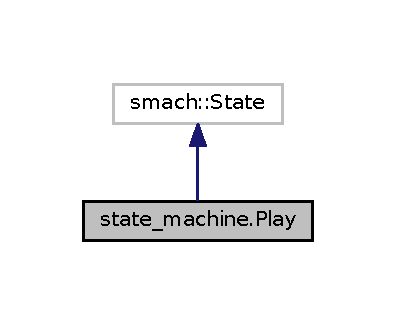
\includegraphics[width=190pt]{classstate__machine_1_1Play__inherit__graph}
\end{center}
\end{figure}


Collaboration diagram for state\+\_\+machine.\+Play\+:
\nopagebreak
\begin{figure}[H]
\begin{center}
\leavevmode
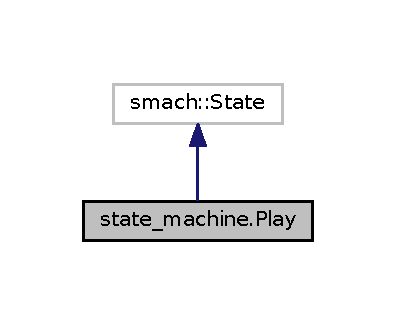
\includegraphics[width=190pt]{classstate__machine_1_1Play__coll__graph}
\end{center}
\end{figure}
\subsection*{Public Member Functions}
\begin{DoxyCompactItemize}
\item 
def \hyperlink{classstate__machine_1_1Play_a5993a23d8be7f7b2647f71ede0334957}{\+\_\+\+\_\+init\+\_\+\+\_\+} (self)
\begin{DoxyCompactList}\small\item\em method init \end{DoxyCompactList}\item 
def \hyperlink{classstate__machine_1_1Play_abf792c51f9931e669b0ed46ba0801986}{robot\+\_\+vel} (self, msg)
\end{DoxyCompactItemize}
\subsection*{Public Attributes}
\begin{DoxyCompactItemize}
\item 
\hyperlink{classstate__machine_1_1Play_a276faca960b7836501ec5e2f0da038a3}{count}
\begin{DoxyCompactList}\small\item\em publishers / subscribers publisher to goal position \end{DoxyCompactList}\item 
\hyperlink{classstate__machine_1_1Play_a1fae7e215371b18cf947e8cd1babb346}{rooms}
\begin{DoxyCompactList}\small\item\em move to command get array containing the list of all Rooms rooms\+: \mbox{[}\textquotesingle{}Room\+Blue\textquotesingle{}, \textquotesingle{}Room\+Red\textquotesingle{}, \textquotesingle{}Room\+Green\textquotesingle{}, \textquotesingle{}Room\+Black\textquotesingle{}, \textquotesingle{}Room\+Magenta\textquotesingle{}, \textquotesingle{}Room\+Yellow\textquotesingle{}\mbox{]} \end{DoxyCompactList}\item 
\hyperlink{classstate__machine_1_1Play_a41a074c4bf967a31676ee879b4522e85}{param}
\begin{DoxyCompactList}\small\item\em switch color \end{DoxyCompactList}\item 
\hyperlink{classstate__machine_1_1Play_a9ffb340aab6992abdb021d3a3aa59099}{go\+To}
\end{DoxyCompactItemize}
\subsection*{Static Public Attributes}
\begin{DoxyCompactItemize}
\item 
\hyperlink{classstate__machine_1_1Play_a60431dacf2811b3dc7e954473c281985}{stop\+Flag}
\end{DoxyCompactItemize}


\subsection{Detailed Description}
class Play\+\_\+behavior 

This class implement the P\+L\+AY behavior of the robot pet It moves the robot to the predefined (X, Y) location within the map and moves it back to the user. The Robot should\+:
\begin{DoxyItemize}
\item start following the ball
\item when the ball stops (it means when the robot stops) it moves the head on the left of 45 degrees, and keep it there for some seconds
\item then it moves the head to the right, stays there for some seconds
\item once moved the head keeps tracking the ball 
\end{DoxyItemize}

\subsection{Constructor \& Destructor Documentation}
\index{state\+\_\+machine\+::\+Play@{state\+\_\+machine\+::\+Play}!\+\_\+\+\_\+init\+\_\+\+\_\+@{\+\_\+\+\_\+init\+\_\+\+\_\+}}
\index{\+\_\+\+\_\+init\+\_\+\+\_\+@{\+\_\+\+\_\+init\+\_\+\+\_\+}!state\+\_\+machine\+::\+Play@{state\+\_\+machine\+::\+Play}}
\subsubsection[{\texorpdfstring{\+\_\+\+\_\+init\+\_\+\+\_\+(self)}{__init__(self)}}]{\setlength{\rightskip}{0pt plus 5cm}def state\+\_\+machine.\+Play.\+\_\+\+\_\+init\+\_\+\+\_\+ (
\begin{DoxyParamCaption}
\item[{}]{self}
\end{DoxyParamCaption}
)}\hypertarget{classstate__machine_1_1Play_a5993a23d8be7f7b2647f71ede0334957}{}\label{classstate__machine_1_1Play_a5993a23d8be7f7b2647f71ede0334957}


method init 

initialization 

\subsection{Member Function Documentation}
\index{state\+\_\+machine\+::\+Play@{state\+\_\+machine\+::\+Play}!robot\+\_\+vel@{robot\+\_\+vel}}
\index{robot\+\_\+vel@{robot\+\_\+vel}!state\+\_\+machine\+::\+Play@{state\+\_\+machine\+::\+Play}}
\subsubsection[{\texorpdfstring{robot\+\_\+vel(self, msg)}{robot_vel(self, msg)}}]{\setlength{\rightskip}{0pt plus 5cm}def state\+\_\+machine.\+Play.\+robot\+\_\+vel (
\begin{DoxyParamCaption}
\item[{}]{self, }
\item[{}]{msg}
\end{DoxyParamCaption}
)}\hypertarget{classstate__machine_1_1Play_abf792c51f9931e669b0ed46ba0801986}{}\label{classstate__machine_1_1Play_abf792c51f9931e669b0ed46ba0801986}


\subsection{Member Data Documentation}
\index{state\+\_\+machine\+::\+Play@{state\+\_\+machine\+::\+Play}!count@{count}}
\index{count@{count}!state\+\_\+machine\+::\+Play@{state\+\_\+machine\+::\+Play}}
\subsubsection[{\texorpdfstring{count}{count}}]{\setlength{\rightskip}{0pt plus 5cm}state\+\_\+machine.\+Play.\+count}\hypertarget{classstate__machine_1_1Play_a276faca960b7836501ec5e2f0da038a3}{}\label{classstate__machine_1_1Play_a276faca960b7836501ec5e2f0da038a3}


publishers / subscribers publisher to goal position 

\index{state\+\_\+machine\+::\+Play@{state\+\_\+machine\+::\+Play}!go\+To@{go\+To}}
\index{go\+To@{go\+To}!state\+\_\+machine\+::\+Play@{state\+\_\+machine\+::\+Play}}
\subsubsection[{\texorpdfstring{go\+To}{goTo}}]{\setlength{\rightskip}{0pt plus 5cm}state\+\_\+machine.\+Play.\+go\+To}\hypertarget{classstate__machine_1_1Play_a9ffb340aab6992abdb021d3a3aa59099}{}\label{classstate__machine_1_1Play_a9ffb340aab6992abdb021d3a3aa59099}
\index{state\+\_\+machine\+::\+Play@{state\+\_\+machine\+::\+Play}!param@{param}}
\index{param@{param}!state\+\_\+machine\+::\+Play@{state\+\_\+machine\+::\+Play}}
\subsubsection[{\texorpdfstring{param}{param}}]{\setlength{\rightskip}{0pt plus 5cm}state\+\_\+machine.\+Play.\+param}\hypertarget{classstate__machine_1_1Play_a41a074c4bf967a31676ee879b4522e85}{}\label{classstate__machine_1_1Play_a41a074c4bf967a31676ee879b4522e85}


switch color 

\index{state\+\_\+machine\+::\+Play@{state\+\_\+machine\+::\+Play}!rooms@{rooms}}
\index{rooms@{rooms}!state\+\_\+machine\+::\+Play@{state\+\_\+machine\+::\+Play}}
\subsubsection[{\texorpdfstring{rooms}{rooms}}]{\setlength{\rightskip}{0pt plus 5cm}state\+\_\+machine.\+Play.\+rooms}\hypertarget{classstate__machine_1_1Play_a1fae7e215371b18cf947e8cd1babb346}{}\label{classstate__machine_1_1Play_a1fae7e215371b18cf947e8cd1babb346}


move to command get array containing the list of all Rooms rooms\+: \mbox{[}\textquotesingle{}Room\+Blue\textquotesingle{}, \textquotesingle{}Room\+Red\textquotesingle{}, \textquotesingle{}Room\+Green\textquotesingle{}, \textquotesingle{}Room\+Black\textquotesingle{}, \textquotesingle{}Room\+Magenta\textquotesingle{}, \textquotesingle{}Room\+Yellow\textquotesingle{}\mbox{]} 

\index{state\+\_\+machine\+::\+Play@{state\+\_\+machine\+::\+Play}!stop\+Flag@{stop\+Flag}}
\index{stop\+Flag@{stop\+Flag}!state\+\_\+machine\+::\+Play@{state\+\_\+machine\+::\+Play}}
\subsubsection[{\texorpdfstring{stop\+Flag}{stopFlag}}]{\setlength{\rightskip}{0pt plus 5cm}state\+\_\+machine.\+Play.\+stop\+Flag\hspace{0.3cm}{\ttfamily [static]}}\hypertarget{classstate__machine_1_1Play_a60431dacf2811b3dc7e954473c281985}{}\label{classstate__machine_1_1Play_a60431dacf2811b3dc7e954473c281985}


The documentation for this class was generated from the following file\+:\begin{DoxyCompactItemize}
\item 
/home/\+Experimental\+Robotics\+Lab\+Serena/src/final\+\_\+assignment/scripts/\hyperlink{state__machine_8py}{state\+\_\+machine.\+py}\end{DoxyCompactItemize}

\hypertarget{classstate__machine_1_1Sleep}{}\section{state\+\_\+machine.\+Sleep Class Reference}
\label{classstate__machine_1_1Sleep}\index{state\+\_\+machine.\+Sleep@{state\+\_\+machine.\+Sleep}}


class Sleep\+\_\+behavior  




Inheritance diagram for state\+\_\+machine.\+Sleep\+:
\nopagebreak
\begin{figure}[H]
\begin{center}
\leavevmode
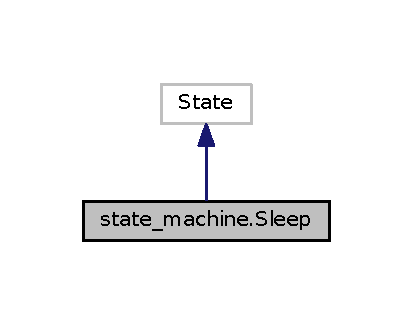
\includegraphics[width=198pt]{classstate__machine_1_1Sleep__inherit__graph}
\end{center}
\end{figure}


Collaboration diagram for state\+\_\+machine.\+Sleep\+:
\nopagebreak
\begin{figure}[H]
\begin{center}
\leavevmode
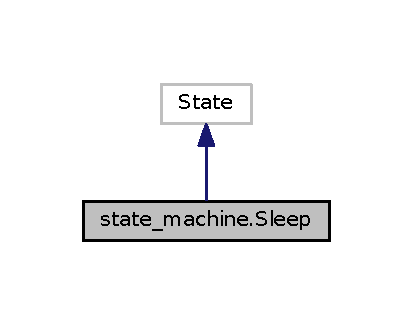
\includegraphics[width=198pt]{classstate__machine_1_1Sleep__coll__graph}
\end{center}
\end{figure}
\subsection*{Public Member Functions}
\begin{DoxyCompactItemize}
\item 
def \hyperlink{classstate__machine_1_1Sleep_a473b93a1ddf11f9e664d1fb694ce1a3c}{\+\_\+\+\_\+init\+\_\+\+\_\+} (self)
\begin{DoxyCompactList}\small\item\em method init \end{DoxyCompactList}\item 
def \hyperlink{classstate__machine_1_1Sleep_a89527836f1edcefb6467fa9c041fbbfe}{execute} (self, userdata)
\item 
def \hyperlink{classstate__machine_1_1Sleep_af89f7f7e1247670de2e6280e3fd1c226}{robot\+\_\+vel} (self, msg)
\begin{DoxyCompactList}\small\item\em method robot\+\_\+vel \end{DoxyCompactList}\end{DoxyCompactItemize}
\subsection*{Static Public Attributes}
\begin{DoxyCompactItemize}
\item 
\hyperlink{classstate__machine_1_1Sleep_a00b879885a7e1f565d91faba0403513d}{stop\+Flag}
\item 
\hyperlink{classstate__machine_1_1Sleep_aaaa470bd53002152ac5b2d3d4ad20c9d}{pub\+Goal} = rospy.\+Publisher(\textquotesingle{}goal\+Pos\textquotesingle{}, Num,queue\+\_\+size=10)
\item 
\hyperlink{classstate__machine_1_1Sleep_a6bd959627ed45867516c94e3eafc05bb}{home} = rospy.\+get\+\_\+param(\textquotesingle{}/home\+Pose\textquotesingle{})
\item 
list \hyperlink{classstate__machine_1_1Sleep_aec191ea286c33d86b339cb95a854ab42}{lista} = \mbox{[}$\,$\mbox{]}
\end{DoxyCompactItemize}


\subsection{Detailed Description}
class Sleep\+\_\+behavior 

This class implement the S\+L\+E\+EP behaviour of the robot pet The robot sleeps (S\+L\+E\+EP state)for a random period of time, then it moves to N\+O\+R\+M\+AL state The robot should\+:
\begin{DoxyItemize}
\item reach a predefined location within the arena in Gazebo
\item stays there for some times
\item go back in N\+O\+R\+M\+AL state 
\end{DoxyItemize}

\subsection{Constructor \& Destructor Documentation}
\index{state\+\_\+machine\+::\+Sleep@{state\+\_\+machine\+::\+Sleep}!\+\_\+\+\_\+init\+\_\+\+\_\+@{\+\_\+\+\_\+init\+\_\+\+\_\+}}
\index{\+\_\+\+\_\+init\+\_\+\+\_\+@{\+\_\+\+\_\+init\+\_\+\+\_\+}!state\+\_\+machine\+::\+Sleep@{state\+\_\+machine\+::\+Sleep}}
\subsubsection[{\texorpdfstring{\+\_\+\+\_\+init\+\_\+\+\_\+(self)}{__init__(self)}}]{\setlength{\rightskip}{0pt plus 5cm}def state\+\_\+machine.\+Sleep.\+\_\+\+\_\+init\+\_\+\+\_\+ (
\begin{DoxyParamCaption}
\item[{}]{self}
\end{DoxyParamCaption}
)}\hypertarget{classstate__machine_1_1Sleep_a473b93a1ddf11f9e664d1fb694ce1a3c}{}\label{classstate__machine_1_1Sleep_a473b93a1ddf11f9e664d1fb694ce1a3c}


method init 

initialization 

\subsection{Member Function Documentation}
\index{state\+\_\+machine\+::\+Sleep@{state\+\_\+machine\+::\+Sleep}!execute@{execute}}
\index{execute@{execute}!state\+\_\+machine\+::\+Sleep@{state\+\_\+machine\+::\+Sleep}}
\subsubsection[{\texorpdfstring{execute(self, userdata)}{execute(self, userdata)}}]{\setlength{\rightskip}{0pt plus 5cm}def state\+\_\+machine.\+Sleep.\+execute (
\begin{DoxyParamCaption}
\item[{}]{self, }
\item[{}]{userdata}
\end{DoxyParamCaption}
)}\hypertarget{classstate__machine_1_1Sleep_a89527836f1edcefb6467fa9c041fbbfe}{}\label{classstate__machine_1_1Sleep_a89527836f1edcefb6467fa9c041fbbfe}
\index{state\+\_\+machine\+::\+Sleep@{state\+\_\+machine\+::\+Sleep}!robot\+\_\+vel@{robot\+\_\+vel}}
\index{robot\+\_\+vel@{robot\+\_\+vel}!state\+\_\+machine\+::\+Sleep@{state\+\_\+machine\+::\+Sleep}}
\subsubsection[{\texorpdfstring{robot\+\_\+vel(self, msg)}{robot_vel(self, msg)}}]{\setlength{\rightskip}{0pt plus 5cm}def state\+\_\+machine.\+Sleep.\+robot\+\_\+vel (
\begin{DoxyParamCaption}
\item[{}]{self, }
\item[{}]{msg}
\end{DoxyParamCaption}
)}\hypertarget{classstate__machine_1_1Sleep_af89f7f7e1247670de2e6280e3fd1c226}{}\label{classstate__machine_1_1Sleep_af89f7f7e1247670de2e6280e3fd1c226}


method robot\+\_\+vel 

callback to check if the robot is moving or not A flag is set to 1 if the robot is not moving, to 0 otherwise 

\subsection{Member Data Documentation}
\index{state\+\_\+machine\+::\+Sleep@{state\+\_\+machine\+::\+Sleep}!home@{home}}
\index{home@{home}!state\+\_\+machine\+::\+Sleep@{state\+\_\+machine\+::\+Sleep}}
\subsubsection[{\texorpdfstring{home}{home}}]{\setlength{\rightskip}{0pt plus 5cm}state\+\_\+machine.\+Sleep.\+home = rospy.\+get\+\_\+param(\textquotesingle{}/home\+Pose\textquotesingle{})\hspace{0.3cm}{\ttfamily [static]}}\hypertarget{classstate__machine_1_1Sleep_a6bd959627ed45867516c94e3eafc05bb}{}\label{classstate__machine_1_1Sleep_a6bd959627ed45867516c94e3eafc05bb}
\index{state\+\_\+machine\+::\+Sleep@{state\+\_\+machine\+::\+Sleep}!lista@{lista}}
\index{lista@{lista}!state\+\_\+machine\+::\+Sleep@{state\+\_\+machine\+::\+Sleep}}
\subsubsection[{\texorpdfstring{lista}{lista}}]{\setlength{\rightskip}{0pt plus 5cm}list state\+\_\+machine.\+Sleep.\+lista = \mbox{[}$\,$\mbox{]}\hspace{0.3cm}{\ttfamily [static]}}\hypertarget{classstate__machine_1_1Sleep_aec191ea286c33d86b339cb95a854ab42}{}\label{classstate__machine_1_1Sleep_aec191ea286c33d86b339cb95a854ab42}
\index{state\+\_\+machine\+::\+Sleep@{state\+\_\+machine\+::\+Sleep}!pub\+Goal@{pub\+Goal}}
\index{pub\+Goal@{pub\+Goal}!state\+\_\+machine\+::\+Sleep@{state\+\_\+machine\+::\+Sleep}}
\subsubsection[{\texorpdfstring{pub\+Goal}{pubGoal}}]{\setlength{\rightskip}{0pt plus 5cm}state\+\_\+machine.\+Sleep.\+pub\+Goal = rospy.\+Publisher(\textquotesingle{}goal\+Pos\textquotesingle{}, Num,queue\+\_\+size=10)\hspace{0.3cm}{\ttfamily [static]}}\hypertarget{classstate__machine_1_1Sleep_aaaa470bd53002152ac5b2d3d4ad20c9d}{}\label{classstate__machine_1_1Sleep_aaaa470bd53002152ac5b2d3d4ad20c9d}
\index{state\+\_\+machine\+::\+Sleep@{state\+\_\+machine\+::\+Sleep}!stop\+Flag@{stop\+Flag}}
\index{stop\+Flag@{stop\+Flag}!state\+\_\+machine\+::\+Sleep@{state\+\_\+machine\+::\+Sleep}}
\subsubsection[{\texorpdfstring{stop\+Flag}{stopFlag}}]{\setlength{\rightskip}{0pt plus 5cm}state\+\_\+machine.\+Sleep.\+stop\+Flag\hspace{0.3cm}{\ttfamily [static]}}\hypertarget{classstate__machine_1_1Sleep_a00b879885a7e1f565d91faba0403513d}{}\label{classstate__machine_1_1Sleep_a00b879885a7e1f565d91faba0403513d}


The documentation for this class was generated from the following file\+:\begin{DoxyCompactItemize}
\item 
/home/\+Experimental\+Robotics\+Lab\+Serena/src/final\+\_\+assignment/scripts/\hyperlink{state__machine_8py}{state\+\_\+machine.\+py}\end{DoxyCompactItemize}

\hypertarget{classstate__machine_1_1state__machine}{}\section{state\+\_\+machine.\+state\+\_\+machine Class Reference}
\label{classstate__machine_1_1state__machine}\index{state\+\_\+machine.\+state\+\_\+machine@{state\+\_\+machine.\+state\+\_\+machine}}


class \hyperlink{classstate__machine_1_1state__machine}{state\+\_\+machine}  


\subsection*{Public Member Functions}
\begin{DoxyCompactItemize}
\item 
def \hyperlink{classstate__machine_1_1state__machine_ac166ab08caa1b688133cda0c9908b244}{\+\_\+\+\_\+init\+\_\+\+\_\+} (self)
\end{DoxyCompactItemize}


\subsection{Detailed Description}
class \hyperlink{classstate__machine_1_1state__machine}{state\+\_\+machine} 

A state machine with 4 states is initialized. 

\subsection{Constructor \& Destructor Documentation}
\index{state\+\_\+machine\+::state\+\_\+machine@{state\+\_\+machine\+::state\+\_\+machine}!\+\_\+\+\_\+init\+\_\+\+\_\+@{\+\_\+\+\_\+init\+\_\+\+\_\+}}
\index{\+\_\+\+\_\+init\+\_\+\+\_\+@{\+\_\+\+\_\+init\+\_\+\+\_\+}!state\+\_\+machine\+::state\+\_\+machine@{state\+\_\+machine\+::state\+\_\+machine}}
\subsubsection[{\texorpdfstring{\+\_\+\+\_\+init\+\_\+\+\_\+(self)}{__init__(self)}}]{\setlength{\rightskip}{0pt plus 5cm}def state\+\_\+machine.\+state\+\_\+machine.\+\_\+\+\_\+init\+\_\+\+\_\+ (
\begin{DoxyParamCaption}
\item[{}]{self}
\end{DoxyParamCaption}
)}\hypertarget{classstate__machine_1_1state__machine_ac166ab08caa1b688133cda0c9908b244}{}\label{classstate__machine_1_1state__machine_ac166ab08caa1b688133cda0c9908b244}


The documentation for this class was generated from the following file\+:\begin{DoxyCompactItemize}
\item 
/home/\+Experimental\+Robotics\+Lab\+Serena/src/final\+\_\+assignment/scripts/\hyperlink{state__machine_8py}{state\+\_\+machine.\+py}\end{DoxyCompactItemize}

\chapter{File Documentation}
\hypertarget{state__machine_8py}{}\section{/home/\+Experimental\+Robotics\+Lab\+Serena/src/final\+\_\+assignment/scripts/state\+\_\+machine.py File Reference}
\label{state__machine_8py}\index{/home/\+Experimental\+Robotics\+Lab\+Serena/src/final\+\_\+assignment/scripts/state\+\_\+machine.\+py@{/home/\+Experimental\+Robotics\+Lab\+Serena/src/final\+\_\+assignment/scripts/state\+\_\+machine.\+py}}
\subsection*{Classes}
\begin{DoxyCompactItemize}
\item 
class \hyperlink{classstate__machine_1_1Normal}{state\+\_\+machine.\+Normal}
\begin{DoxyCompactList}\small\item\em class Normal\+\_\+behavior \end{DoxyCompactList}\item 
class \hyperlink{classstate__machine_1_1Sleep}{state\+\_\+machine.\+Sleep}
\begin{DoxyCompactList}\small\item\em class Sleep\+\_\+behavior \end{DoxyCompactList}\item 
class \hyperlink{classstate__machine_1_1Play}{state\+\_\+machine.\+Play}
\begin{DoxyCompactList}\small\item\em class Play\+\_\+behavior \end{DoxyCompactList}\item 
class \hyperlink{classstate__machine_1_1Find}{state\+\_\+machine.\+Find}
\begin{DoxyCompactList}\small\item\em class Find\+\_\+behavior \end{DoxyCompactList}\item 
class \hyperlink{classstate__machine_1_1state__machine}{state\+\_\+machine.\+state\+\_\+machine}
\begin{DoxyCompactList}\small\item\em class \hyperlink{classstate__machine_1_1state__machine}{state\+\_\+machine} \end{DoxyCompactList}\end{DoxyCompactItemize}
\subsection*{Namespaces}
\begin{DoxyCompactItemize}
\item 
 \hyperlink{namespacestate__machine}{state\+\_\+machine}
\item 
 \hyperlink{namespacebehavior__manager}{behavior\+\_\+manager}
\begin{DoxyCompactList}\small\item\em Here is implemented the state machine that controls the switch between the behaviours of the robot. \end{DoxyCompactList}\end{DoxyCompactItemize}
\subsection*{Functions}
\begin{DoxyCompactItemize}
\item 
def \hyperlink{namespacestate__machine_abbdd360e43abe493ed21338d848f100f}{state\+\_\+machine.\+user\+\_\+action} (data)
\begin{DoxyCompactList}\small\item\em function user\+\_\+action \end{DoxyCompactList}\item 
def \hyperlink{namespacestate__machine_ad624b5f98b8358f20b7cecc4b88c9f52}{state\+\_\+machine.\+random\+\_\+position} ()
\begin{DoxyCompactList}\small\item\em function random\+\_\+position \end{DoxyCompactList}\end{DoxyCompactItemize}
\subsection*{Variables}
\begin{DoxyCompactItemize}
\item 
tuple \hyperlink{namespacestate__machine_aa0d3e8fce4b6fe8788f035c40482a6c6}{state\+\_\+machine.\+green\+Lower} = (50, 50, 20)
\begin{DoxyCompactList}\small\item\em define colours limits for Open\+CV algorithm in our simulation we have different colourd balls\+: green, black, red, yellow, blue, magenta $\ast$$\ast$$\ast$ green $\ast$$\ast$$\ast$ \end{DoxyCompactList}\item 
tuple \hyperlink{namespacestate__machine_adf0d73f9e376e0b066d4ab6127dc498b}{state\+\_\+machine.\+green\+Upper} = (70, 255, 255)
\item 
tuple \hyperlink{namespacestate__machine_ae800938b579cd16f85cdd743d58143e5}{state\+\_\+machine.\+black\+Lower} = (0, 0, 0)
\item 
tuple \hyperlink{namespacestate__machine_a07afd0b9efebc18e612ffbf6f0d729ca}{state\+\_\+machine.\+black\+Upper} = (5, 50, 50)
\item 
tuple \hyperlink{namespacestate__machine_a4905a105f2253662020e49c78e77312a}{state\+\_\+machine.\+red\+Lower} = (0, 50, 50)
\item 
tuple \hyperlink{namespacestate__machine_aa2123f5d6cb9631ca61253c0a17ce023}{state\+\_\+machine.\+red\+Upper} = (5, 255, 255)
\item 
tuple \hyperlink{namespacestate__machine_a8e2b229e1bd3bd9d87cf71403c018b70}{state\+\_\+machine.\+yellow\+Lower} = (25, 50, 50)
\item 
tuple \hyperlink{namespacestate__machine_a483ae42836541d8b86afd10162b39814}{state\+\_\+machine.\+yellow\+Upper} = (35, 255, 255)
\item 
tuple \hyperlink{namespacestate__machine_a0410a5010d534f980f7b6690b58961da}{state\+\_\+machine.\+blue\+Lower} = (100, 50, 50)
\item 
tuple \hyperlink{namespacestate__machine_acaae31790ee8ca5aedbf802044e5c489}{state\+\_\+machine.\+blue\+Upper} = (130, 255, 255)
\item 
tuple \hyperlink{namespacestate__machine_ac525748b3dd0fe5a7626ca96597c7137}{state\+\_\+machine.\+magenta\+Lower} = (125, 50, 50)
\item 
tuple \hyperlink{namespacestate__machine_aba747bf4284a6a4eb77a1935875efe95}{state\+\_\+machine.\+magenta\+Upper} = (150, 255, 255)
\end{DoxyCompactItemize}

%--- End generated contents ---

% Index
\backmatter
\newpage
\phantomsection
\clearemptydoublepage
\addcontentsline{toc}{chapter}{Index}
\printindex

\end{document}
